\documentclass{report}
\usepackage{amsmath}
\usepackage{graphicx}
\usepackage{listings}
\usepackage[a4paper, margin=0.5in]{geometry}
\usepackage{xcolor}
\usepackage{newtxmath}
\usepackage{tcolorbox}
\usepackage{float}
\usepackage{chngcntr}
\usepackage{tikz}
\usepackage{pgfplots}
\usetikzlibrary{matrix,chains,positioning,decorations.pathreplacing,arrows}

\counterwithin{figure}{section}
\counterwithin{equation}{section}


\title{Predicting flow with Back Propagation Neural Networks}
\author{F328799}
\date{}

% Define the code style %
\definecolor{codegreen}{HTML}{3d405b}
\definecolor{codegray}{rgb}{0.5,0.5,0.5}
\definecolor{codepurple}{HTML}{e07a5f} 
\definecolor{keycolour}{HTML}{81b29a}

\definecolor{contextback}{HTML}{f1faee}
\definecolor{contextframe}{HTML}{81b29a}


\lstdefinestyle{codeStyle}{
    commentstyle=\color{codegreen},
    keywordstyle=\color{keycolour},
    numberstyle=\tiny\color{codegray},
    stringstyle=\color{codepurple},
    basicstyle=\ttfamily\footnotesize\fontfamily{ptm}\selectfont,
    breakatwhitespace=false,         
    breaklines=true,                 
    captionpos=b,                    
    keepspaces=true,                 
    numbers=left,                    
    numbersep=5pt,                  
    showspaces=false,                
    showstringspaces=false,
    showtabs=false,                  
    tabsize=2
}

\lstset{style=codeStyle}

\tcbset{
    contextnote/.style={
        colback=contextback, % Background color
        colframe=contextframe, % Border color
        fonttitle=\bfseries, % Title font
        coltitle=black, % Title color
        colbacktitle=yellow!50!white, % Title background color
        coltext=black, % Text color
        fontupper=\itshape, % Italic text
        boxrule=0.5mm, % Border thickness
        arc=1mm, % Rounded corners
    }
}


\begin{document}
\maketitle

\tableofcontents

\setcounter{chapter}{-1} % start chapter numbering at 0 %
\chapter{Outline} % explain the aims of the project %
The aim of this project is to predict the flow-rate of the River Ouse at Skelton in advance to predict the flood potential.
We will use a Back Propagation Neural Network to predict the flow-rate of the river, using data from the surrounding catchment area.
This data includes river flow-rate from Skip Bridge, Crakehill and Westwick, as well as rainfall data from East Cowton, Arkengarthdale, Snaizeholme and Malham Tarn.
The data was collected between 01/01/1993 to 31/12/1996.

\begin{figure}[H]
    \centering
    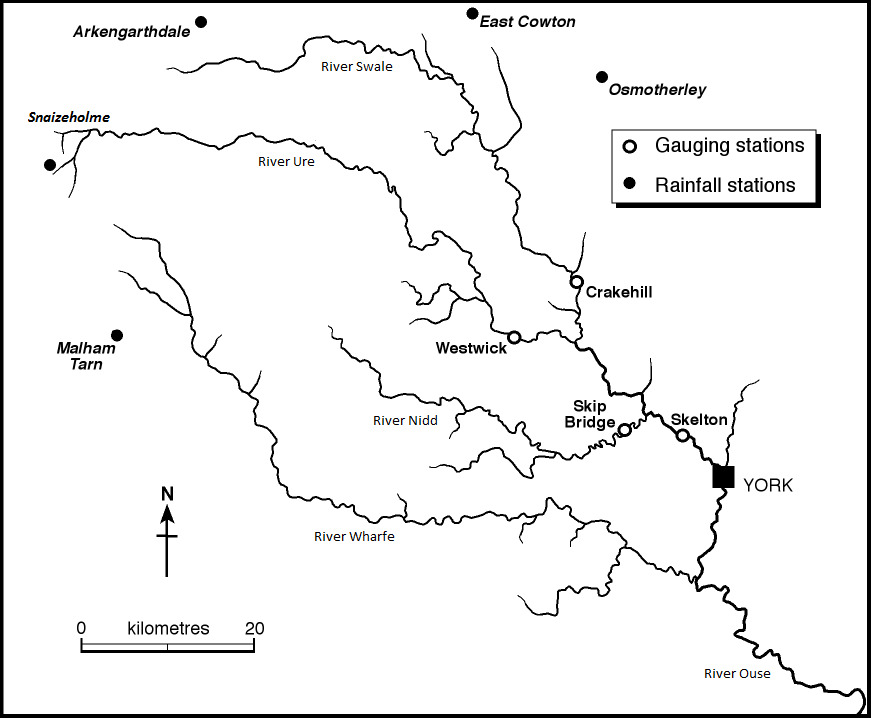
\includegraphics[width=0.7\textwidth]{images/river_ouse.jpg} % Replace with the correct path to your image
    \caption{River Ouse Catchment}
    \label{fig:river_ouse}
\end{figure}

The sections of this report will include:
\begin{enumerate}
    \item Data Pre-processing
    \item Implementing the Neural Network
    \item Model Training
    \item Evaluation
\end{enumerate}

\section{System Environments}
The ANN will be programmed using python 3.13.2 with a conda virtual environment.
The libraries used will include:
\begin{itemize}
    \item numpy
    \item pandas, sqlalchemy
    \item openpyxl
    \item sqlite3
    \item matplotlib
    \item seaborn
    \item time
    \item matplotlib's PdfPages
\end{itemize}

The data will be stored in an SQLite database, this is for ease of access and to keep the data in a single location, with concise SQL commands to access the data.

\chapter{Data Pre-processing}
\section{Importing data}

The first step is to import the data from the give xlsx file into the database.
This will be done using the pandas library to read the data from the xlsx file and then using the sqlalchemy library to write the data to the database.
For simplicity, I created a second xlsx file without the first row of headers, this is so that the data can be read into the database without any issues.
\vspace{1em}
\newline
This code shows how I handled the non-numerical data in the xlsx file.
It is then imported into the database using the sqlalchemy library.
Line 16 is used to remove non-numerical data when importing into the database.
This is to avoid any type-errors when the create\_engine creates the dataBase.
\begin{lstlisting}[language=Python] 
excel_import.py

    import pandas as pd
    import numpy as np
    import sqlite3 
    from sqlalchemy import create_engine
    
    
    def data_import(dataBase:pd.DataFrame, dataTable:str, excelFile:str):
        '''Function for importing Excel data into a database'''

        # Read the excel file and store the data in a DataFrame
        excelFile = pd.read_excel(excelFile)

        # Check for non-numeric values in non-first columns and replace them with na points
        excelFile.iloc[:, 1:] = excelFile.iloc[:, 1:].apply(pd.to_numeric, errors='coerce').fillna(np.nan)

        # Create a connection to the SQLite database (or create it if it doesn't exist)
        conn = sqlite3.connect(dataBase)
        cursor = conn.cursor()

        # Drop the table if it exists so the database can be recreated from scratch for testing
        cursor.execute(f'DROP TABLE IF EXISTS {dataTable}')

        # Use SQLAlchemy to import the DataFrame into the SQL database
        engine = create_engine(f'sqlite:///{dataBase}')
        excelFile.to_sql(dataTable, engine, if_exists='replace', index=False)

        # Commit the changes and close the connection
        conn.commit()
        conn.close()
        print('Data imported successfully!')

\end{lstlisting}
All code will be enclosed in the additional files included 
\vspace{1em}

\section{Extreme Outliers}
Using the database as a source of data, we can now begin to pre-process the data.
Using matplotlib, we can plot the data to see if there are any trends or patterns in the data,
along with any outliers that may need to be removed.

\vspace{1em}
In the given dataset, there were a number of values that were not possible, such as negative flow rates and rainfall values in the thousands.
These values need to be removed from the dataset to ensure the model is accurate.
To remove these and other 'extreme' outliers, I used the inter-quartile range (IQR) method.
When I implemented this, I used a variable to multiply by the IQR to get the upper and lower bounds, allowing me to refine the data to a point I thought was acceptable.

\vspace{1em}
A typical weight for extreme values is 3, this is because the IQR is the range between the 25th and 75th percentile, so multiplying by 3 gives a range of 99.7\% of the data (when its normally distributed).
However, as the data is skewed heavily towards 0, the 75th percentile still encapsulates a large amount of possible data within a wide range.
After experimenting with different values, the results were as follows:

\begin{table}[h]
    \centering
    \begin{tabular}{|c|c|}
        \hline
        Weight & Amount Removed \\
        \hline
        1.5 & 2031 \\
        3.0 & 782 \\
        6.0 & 176 \\
        10.0 & 50 \\
        \hline
    \end{tabular}
    \caption{Results of different weights for IQR}
    \label{tab:iqr_results}
\end{table}

From testing, I decided that 10 was the best weight to use, as it removed the most extreme values without removing too much data.
The remaining data looks real and is within a reasonable range for realistic rainfall and flow rates.

\section{Averaging and Deviations}

The data has had its extreme outliers removed, but it is still not in a usable state.
The data needs to be averaged and standardised to ensure that the data is in a usable state for the neural network.

\begin{tcolorbox}[contextnote]
    For context:
These functions are called within an iterative loop that acts on them for each of the columns in the database.
columnData is a pandas data frame of the date with that dates record.
\vspace{1em}
\newline
The data points are uniformly iterated with columnData.itertuples(), hence the use of the point[n] convention to access the data.
\vspace{1em}
\newline
When a data point is removed, it is stored in a dictionary object, with the key being the column name and the value being a dictionary of the removed data points.
All code will be enclosed in the additional files included.
\end{tcolorbox}
\vspace{1em}
Our IQR with extreme weighting method does not account for large amount of rainfall in a dry spell, or low flow rate at a time of flooding.
To account for this, we will use methods to determine if the data is within a reasonable range, over a period of time.
\vspace{1em}
\newline
Rainfall and especially flow rate data move in trends, so to best capture the data we will use a condensed version of the data, with only its neighbors.
We will calculate our outliers over this as rainfall in summer will not be as high as in winter (it's still England though), so calculating the averages of the whole data set will not be accurate.
\begin{lstlisting}[language=Python]
data_cleaning.py

    import numpy as np
    import pandas as pd

    def local_range_df(columnData:pd.DataFrame, dataPoint:tuple, columnLength:int, windowSize:int) -> pd.DataFrame:
        '''Function to create a smaller range of data around a point'''
        windowSplit = round(windowSize/2)

        # Defines the start and end of the range
        if int(dataPoint[0])-windowSplit < 0:
            '''If the point is close to 0'''
            start = 0
            end = windowSize-int(dataPoint[0])
        elif int(dataPoint[0])+windowSplit > columnLength:
            '''If the point is close to the end of the DF'''
            end = columnLength
            start = columnLength - windowSize
        else:
            '''If the point is in the middle of the DF'''
            start = int(dataPoint[0])-windowSplit
            end = int(dataPoint[0])+windowSplit

        # Create a range of the data around the point
        localData = columnData.loc[start:end]

        return localData
\end{lstlisting}
We will pass this local data to the standard deviation and IQR functions to calculate the upper and lower bounds of the data.
\vspace{1em}
\newline
Flow rate of a river rises and falls in patterns, so to best catch outliers we will use a mean and standard deviation over a period of time.
\begin{lstlisting}[language=Python] 
data_cleaning.py

    import numpy as np
    import pandas as pd

    def standard_deviation_calculator(columnData:pd.DataFrame, columnName:str, deviationWeight:int) -> tuple[float, float]:
        '''Function to calculate the standard deviation of a range of data'''

        # Calculate the mean and standard deviation of the DataFrame
        deviation = columnData[columnName].std(axis=0, skipna=True, numeric_only=True, ddof=1)
        average = columnData[columnName].mean(axis=0, skipna=True, numeric_only=True)

        # Calculate the upper and lower bounds
        lowerBound = average - (deviationWeight * deviation)
        upperBound = average + (deviationWeight * deviation)

        return lowerBound, upperBound


\end{lstlisting}
This method determines if the data follows the trend of its neighbors, and if it does not, it is removed from the dataset.
One day of high flow rate isn't a realistic measurement as the river constantly flows.
\vspace{1em}
\newline
However, rainfall can be more sporadic, so we will once again use a weighted IQR method to remove extreme values.
\begin{lstlisting}[language=Python] 
data_cleaning.py
    
    import numpy as np
    import pandas as pd

    def iqr_calculator(columnData:pd.DataFrame, columnName:str, deviationWeight:int) -> tuple[float, float]:
        '''Function to calculate the IQR of a range of data'''

        # Calculate the IQR of the range
        Q1 = columnData[columnName].quantile(0.25)
        Q3 = columnData[columnName].quantile(0.75)
        IQR = Q3 - Q1

        # Calculate the upper and lower bounds, round to 3 decimal places
        lowerBound = round(Q1 - (deviationWeight * IQR), 3)
        upperBound = round(Q3 + (deviationWeight * IQR), 3)

        return lowerBound, upperBound

        
\end{lstlisting}
This will be done over a period of time, as a single day of high rainfall is possible in a storm, before a low rainfall spell occurs again.
By splitting the data this way we allow the more accurate flow rate data to be used in the model, while still allowing for the sporadic nature of rainfall.
\vspace{1em}
\newline
Once the data points have been removed from the dataset, we can replace them with the average of the surrounding data points.
This is to ensure that the data is continuous and that the model can be trained on the data.

\section{Interpolation}

When the algorithm removes the data points, it leaves gaps in the data.
I made this decision to separate the extraction and interpolation for two reasons:
\begin{enumerate}
    \item To allow for efficiency of interpolation
    \item For accuracy, as im only using the data points that were recorded, not interpolated
\end{enumerate}

To interpolate the data, I used a simple moving average (SMA) method to fill the gaps.
I implemented this with a variable window size for the SMA to allow for flexibility in the data.
The numpy array allows for skipping of NaN values, so the data can be interpolated in places where I have removed the data points.
However, too small of a window size ends up with a variation of a forward fill at points with data removed.
I decided that a window size of 6 was the best for the data, allowing for trends to show without ending up with a forward fill.

\begin{lstlisting}[language=Python]
data_cleaning.py
 
    import numpy as np
    import pandas as pd

    def simple_moving_average(columnData:pd.DataFrame, columnName:str, windowSize:int, removedDict:dict, updatedDict:dict) -> tuple[dict, dict]:
        '''Function to update empty points in the dataset'''

        # Find all NaN values in the column
        emptyPoints = columnData[columnData[columnName].isna()]

        # Iterate through the empty points
        for point in emptyPoints.itertuples():
            '''Iterate through the empty points in the DataFrame'''

            # Get the local range of data around the point
            localData = local_range_df(columnData, point, len(columnData), windowSize)

            # Calculate the average of the range
            average = round(localData[columnName].mean(skipna=True),)

            # Update the statistics
            removedDict[columnName][point[1]].append(float(average))

            # For visualisation purposes, store some of the updated data in separate dictionary
            try:
                updatedDict[columnName][point[1]].append(float(average))
            except:
                None

            # Replace the empty point with the average
            columnData.loc[point[0], columnName] = average

        return removedDict, updatedDict
\end{lstlisting}
The outputs of this function are two dictionary objects.
As explained in the context note, the dictionary is used to store the data points that were removed from the dataset.
Both of them are the same, except updatedDict is used for visualisation purposes.
As the extreme values are present in the removedDict, when plotted they skew the graph so you can't see the trends in the data.
\vspace{1em}
\newline
I then go on to use the updatedDict to plot the data, showing the trends in the data, along with the removed data and the ones that replaced it.
This is to show the accuracy of the interpolation and to show the trends in the data.
The removedDict is used to update the SQL database, so the data can be used in the neural network; we need a record of data that was changed to be able to update it.
If we instead saved it to the data frame, we would lose the location of updated data points.
This would result in updating the whole database with the whole data frame, wasting a lot of time and resources replacing points with values they already have.
The database has 11,688 data points, with 992 (for variables stated in figure 1.5.2) removed and replaced. That's 8.5\% of the data and more than 10 times more efficient only updating those.
\section{Plotting trends}
Once the data has been cleaned and interpolated, we can plot the data to see the trends in the data.
We can also make judgments on the variables that determine which point are outliers and which are not.

Lets use the data at Crakehill as an example location for visualisation:
\vspace{1em}
\newline
Figure 1.5.1 show us the data at Crakehill, with the unrealistic data present.
As I stated before, the data scale is affected by the outliers, so the trends in the data are not visible.

\begin{figure}[H]
    \centering
    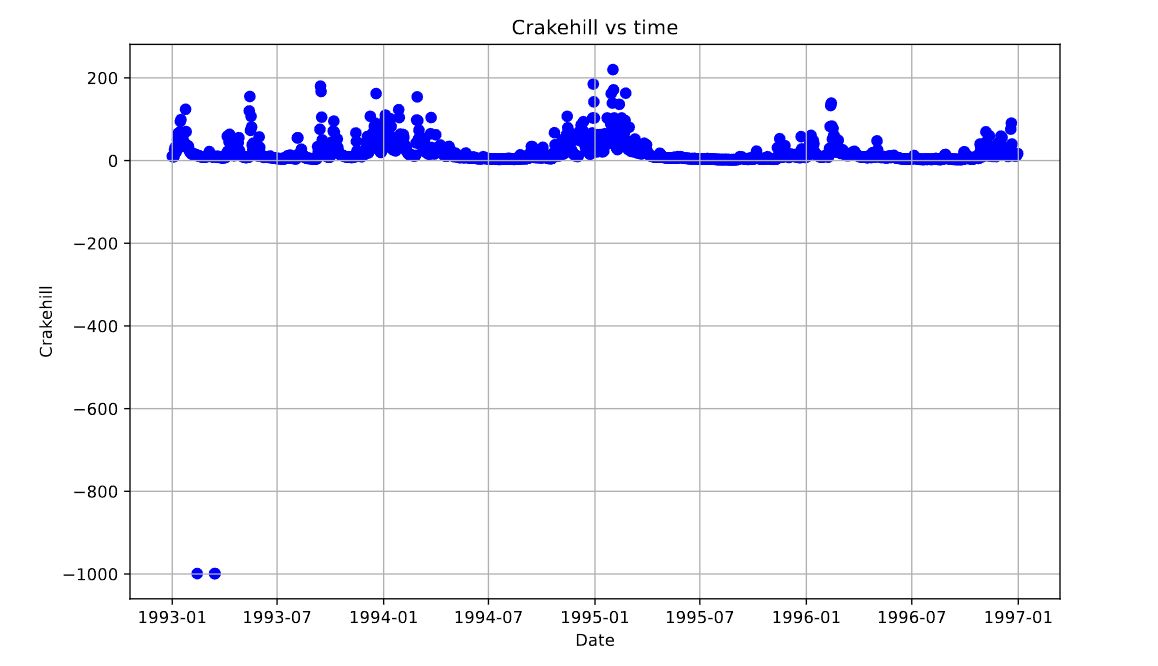
\includegraphics[width=0.7\textwidth]{images/CH_outliers.png}
    \caption{Crakehill Data with unrealistic data}
    \label{fig:Crakehill_outliers}
\end{figure}
\vspace{1em}
Figure 1.5.2 shows the data at Crakehill, with the unrealistic data points removed, but still containing outliers
\begin{figure}[H]
    \centering
    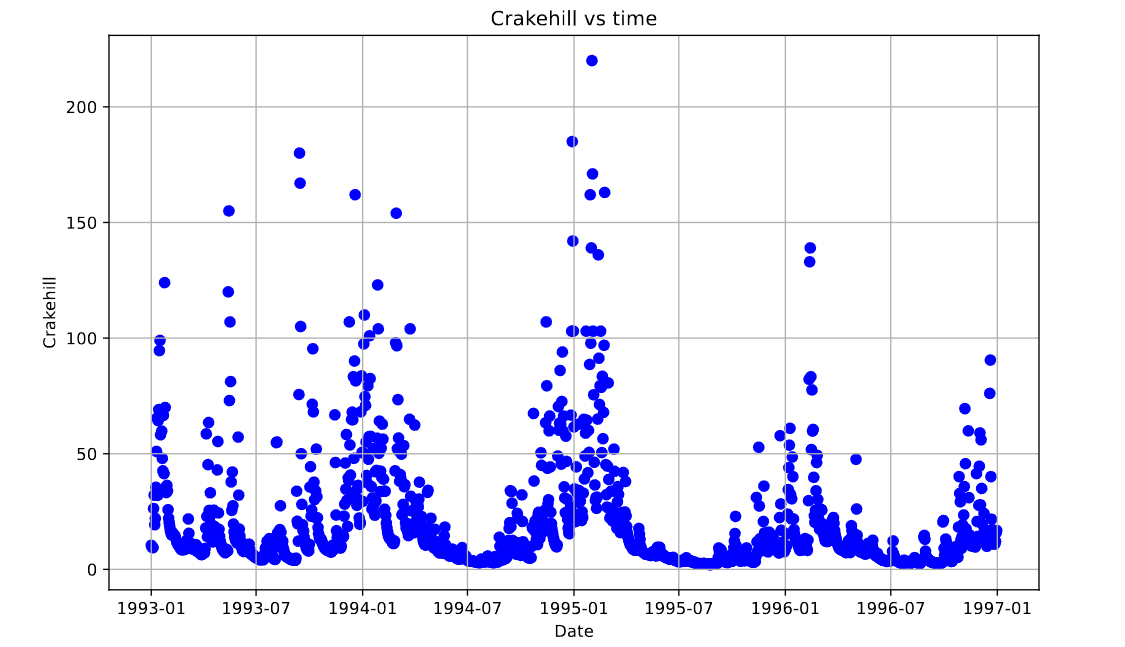
\includegraphics[width=0.7\textwidth]{images/CH_no_outliers.png} 
    \caption{Crakehill Data without unrealistic data}
    \label{fig:Crakehill_no_outliers}
\end{figure}
\vspace{1em}
Finally, figure 1.5.3 shows us the result of our interpolation, with the data points that were removed and replaced.
Blue points are the data we are using, red points are the data that was removed and green being what replaced them.
\begin{figure}[H]
    \centering
    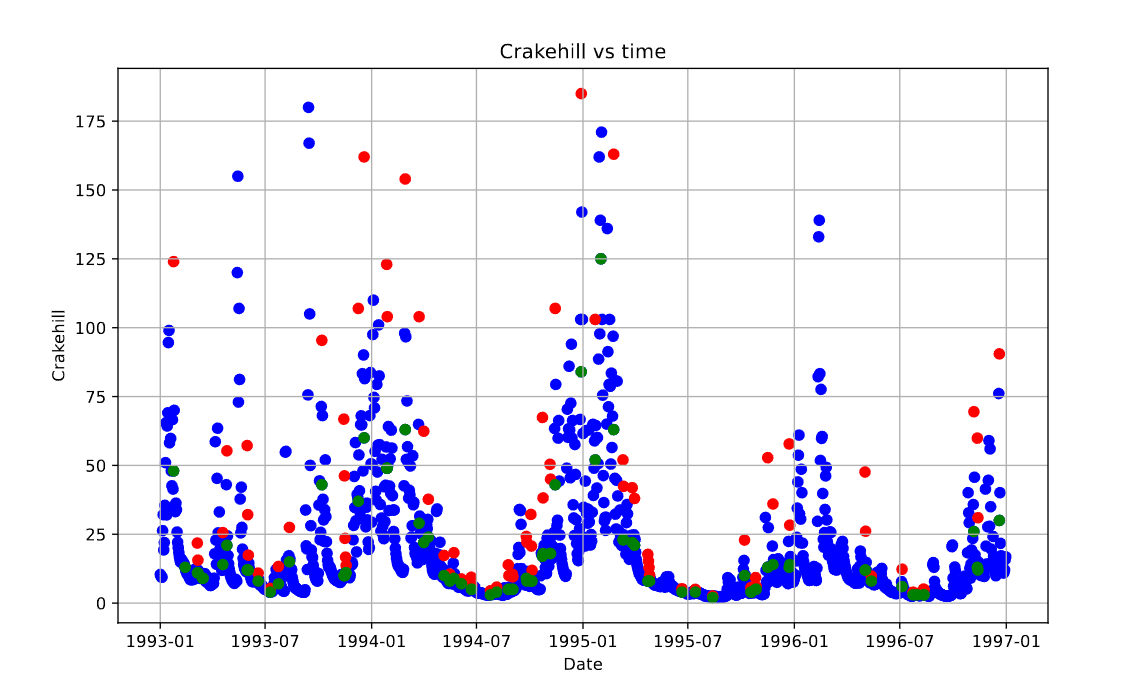
\includegraphics[width=0.7\textwidth]{images/CH_interploated_1.png}
    \caption{Crakehill Data interpolated}
    \label{fig:Crakehill_interpolated_1}
\end{figure}
This specific figure has:
\begin{itemize}
    \item IQR weight of 1.5
    \item Standard deviation weight of 2
    \item Window size of 10 for removal
    \item Window size of 6 for interpolation
    \item 91 data points removed and replaced (992 across all locations)
\end{itemize}
When looking at figure 1.5.2, we can see that in 1993, the flow rate data was much more sporadic than the following years, then in figure 1.5.3, the data is clearly less sporadic and follows the trends more closely.
This data should now be considered usable to train our Multi-Layer Perceptron (MLP) model.
The database can now be updated with the new data.

\section{Correlation}
To best predict our data, we need to choose the correct inputs that will give us the best results.
We need to aim to a high correlation of the data points to the predictand, while also avoiding correlation between predictors.
\begin{figure}[H]
    \centering
    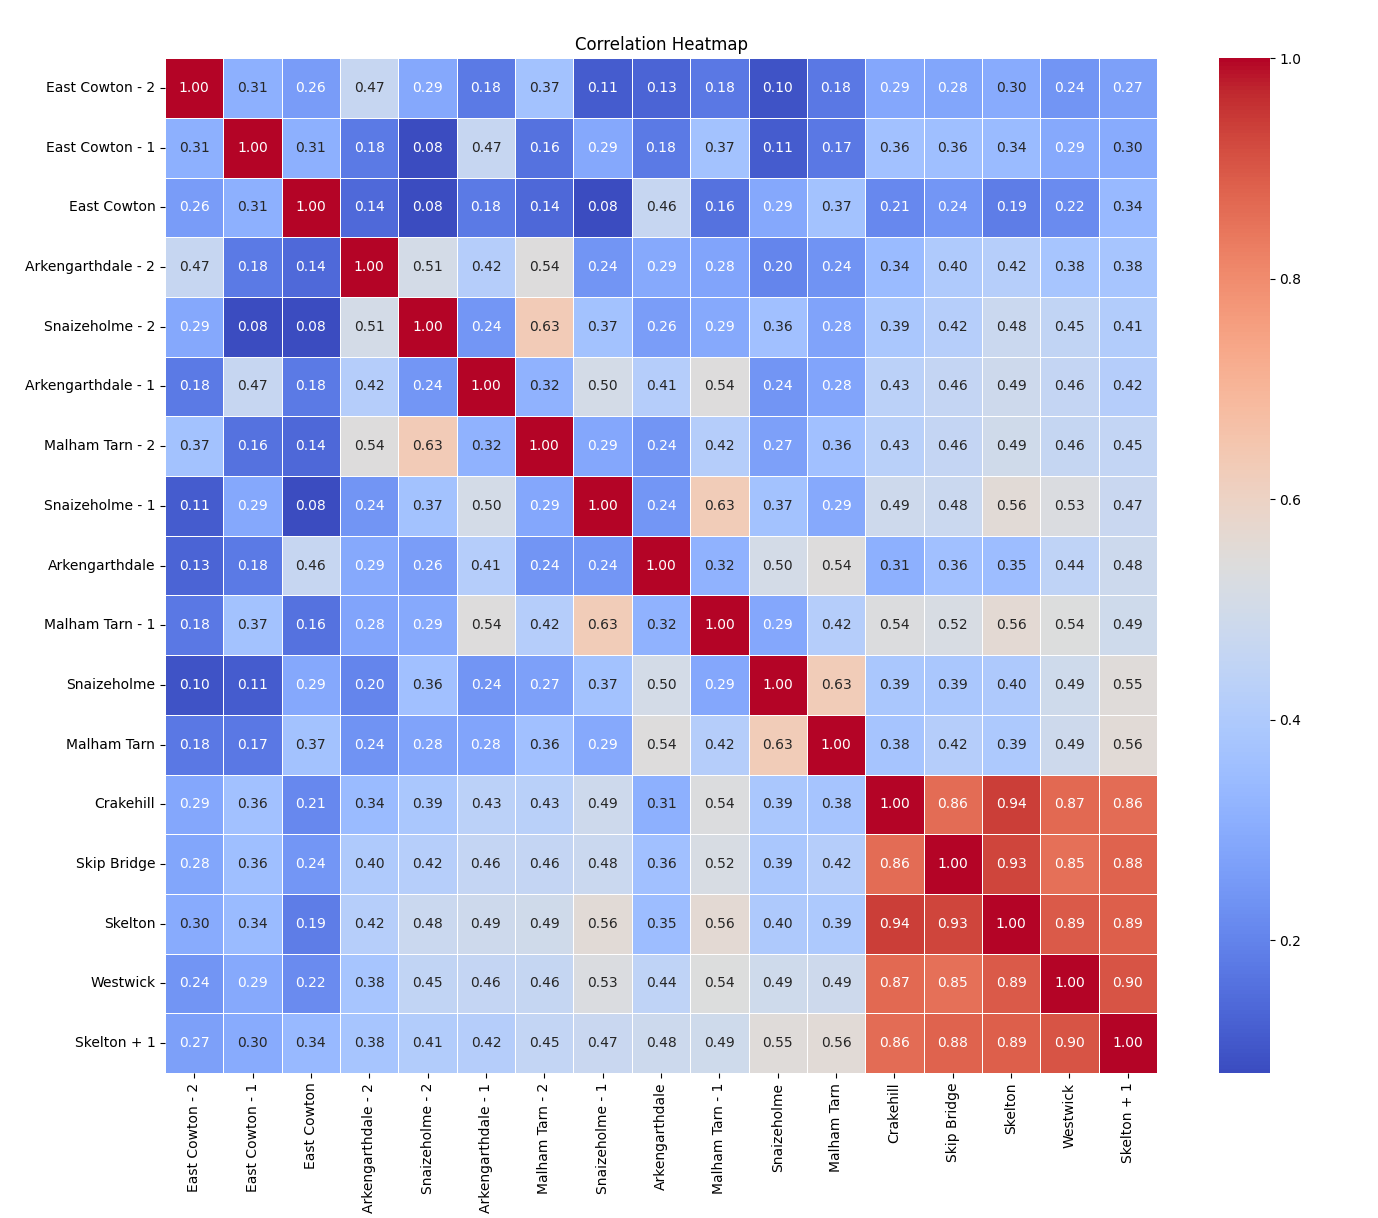
\includegraphics[width=0.9\textwidth]{images/correlation.png}
    \caption{Correlation between the data points}
    \label{fig:correlation}
\end{figure}
FIgure 1.6.1 shows the correlation between the data points, which we can use to determine the best predictors for our model.
As we are trying to to predict the flow rate at Skelton for the day after a data point, the correlation map has been ordered by the correlation to Skelton + 1.
The highest correlation points are the other flow rate data points, with the highest being the flow rate at Westwick.
They are all highly correlated to Skelton +1, but also to each other. This is to be expected as they are all flow rate data points of the same river.
An interesting point to note is that Westwick is the least correlated to Skelton on the day of measurement, but most correlated to the day after.
\vspace{1em}
\newline
The rainfall data is much less correlated to the flow rate data, with the highest correlation being 0.56 at Malham Tarn.
This is to be expected as the rainfall data is not directly related to the flow rate data, but the flow rate data is related to the rainfall data.
The next highest correlated rainfall location is Snaizeholme (0.55), but this also has a high correlation to Malham Tarn.
Refering back to figure 0.0.1, we can see that they are very close, and therefore the data will be very similar.
\newline
The next best correlations are at Malham Tarn -1 (0.49) and Arkengarthdale(0.48), but these are are not nearly as correlated each other and the previous two.
\vspace{1em}
\newline
My initial choice for predictors will be Westwick, Snaizeholme and Malham Tarn-1, as they are the most correlated to Skelton +1, but also the least correlated to each other.
Another option for predictors would be any of the other flow rate data points, and a combination of the 4 mentioned rainfall data points.
\vspace{1em}
\newline
We can also use some more complex predictors to see if they are more correlated to the predictand.
These complex predictors will be using averages of the data points, and adding select ones together to get a higher correlation.
\newline
\begin{figure}[H]
    \centering
    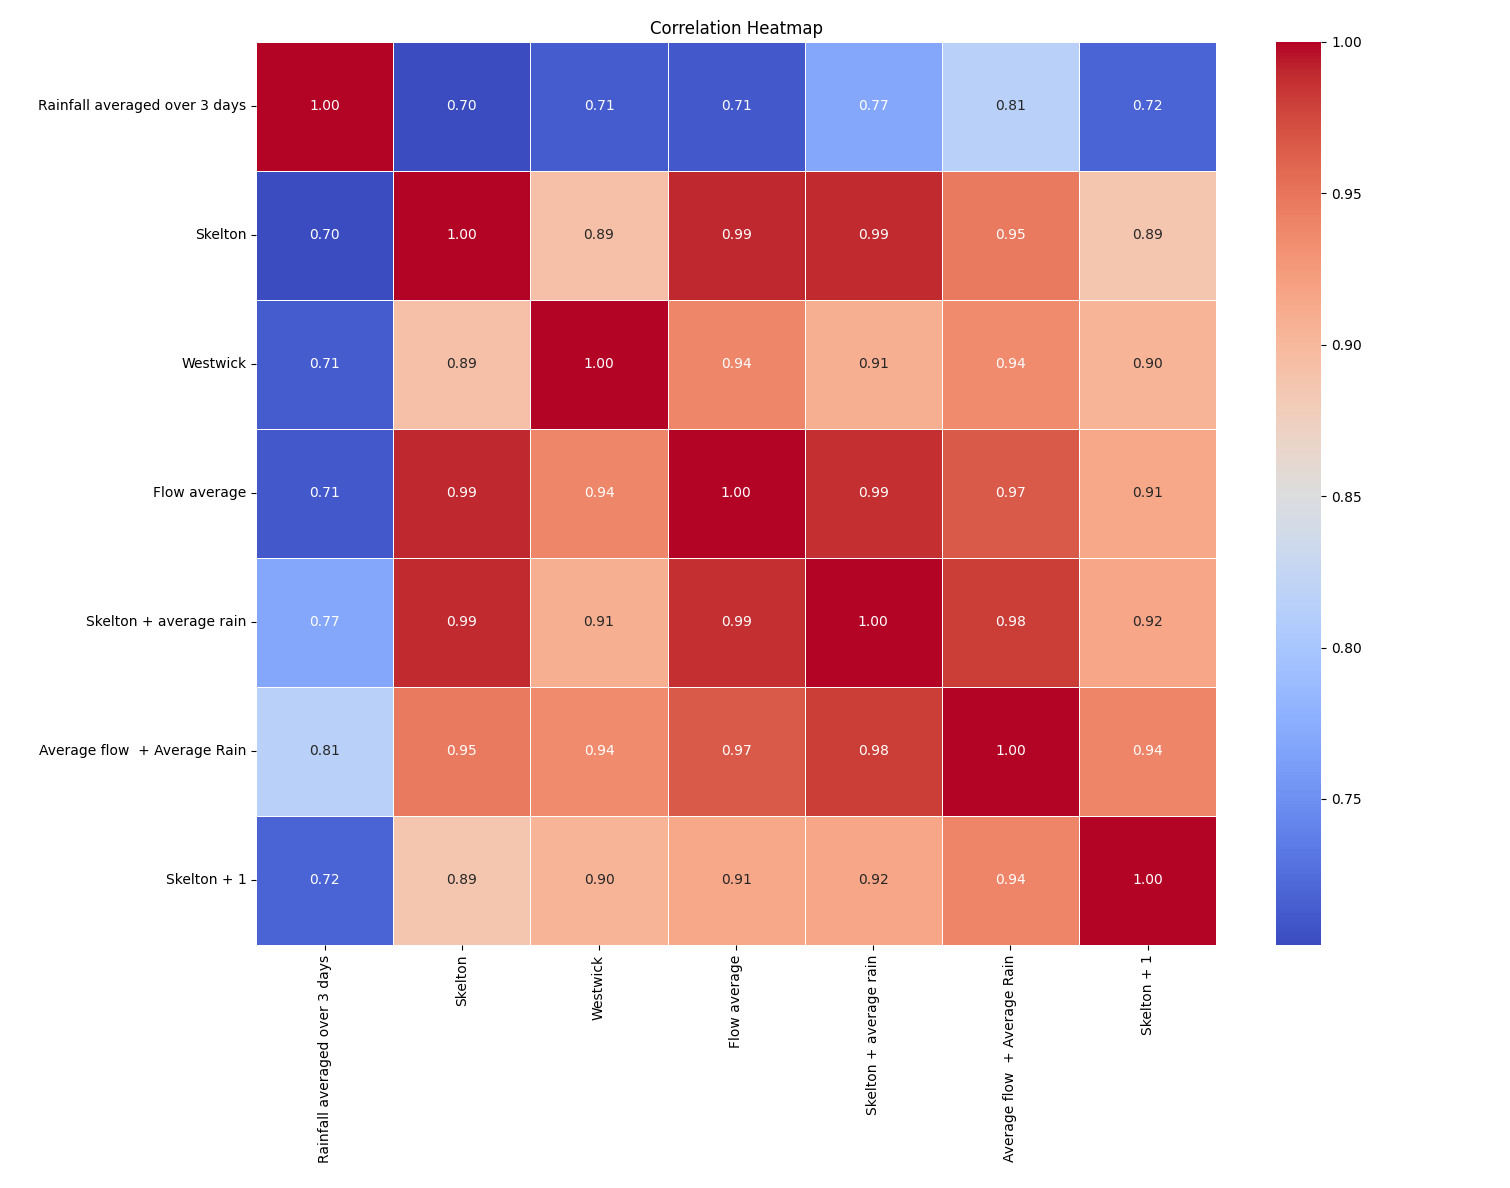
\includegraphics[width=0.9\textwidth]{images/correlation2.png}
    \caption{Complex Correlation between the data points}
    \label{fig:correlation}
\end{figure}
Figure 1.6.2 shows some of the selected complex data points. 
In a network of this size, the correlation between points is not as important as the correlation to the predictand, however I don't want to derive complex points that are too mathematically similar to one another.
\begin{lstlisting}[language=Python]
correlation_mapping.py

import pandas as pd
import seaborn as sns
import matplotlib.pyplot as plt
import reading_and_writing as rw

# Read the data
dataFrame = rw.read_data_all(dataBase, dataTable).iloc[:, 1:]

# Formulate the complex predictors
correlationTable['Skelton + 1'] = dataFrame['Skelton'].shift(-1)
correlationTable['Average flow  + Average Rain'] = (dataFrame['Flow average'] + dataFrame['Rainfall average'])
correlationTable['Skelton + average rain'] = (dataFrame['Skelton'] + dataFrame['Rainfall average'])
correlationTable['Flow average'] = (dataFrame['Skelton'] + dataFrame['Westwick'] + dataFrame['Skip Bridge'] + dataFrame['Crakehill']) / 4
correlationTable['Westwick'] = (dataFrame['Westwick'])
correlationTable['Skelton'] = dataFrame['Skelton']
correlationTable['Rainfall averaged over 3 days'] = dataFrame['Rainfall average'] + dataFrame['Rainfall average -1'] + dataFrame['Rainfall average -2']

# Drop na values
correlationTable = correlationTable.dropna()

# Calculate the correlation matrix
correlationMatrix = correlationTable.corr()

# Sort the correlation matrix
correlationMatrix = correlationMatrix.sort_values(by='Skelton + 1', axis=0, ascending=True)
correlationMatrix = correlationMatrix.sort_values(by='Skelton + 1', axis=1, ascending=True)


# Plot the correlation matrix
plt.figure(figsize=(16, 12))
sns.heatmap(correlationMatrix, annot=True, cmap='coolwarm', fmt=".2f", linewidths=0.5)
plt.title("Correlation Heatmap")
plt.show()

\end{lstlisting}


\chapter{Implementing the Neural Network}
The neural network will be implemented using python and trained with the back propagation algorithm.
The network will be a multi-layer perceptron (MLP), with at least one hidden layer.
\vspace{1em}
\newline
Back propagation works by calculating the expected output of a network, then comparing it to the actual output; this is known as the forward pass.
The algorithm then works backwards through the network, adjusting the weights of the network to reduce the error between the expected and actual output - the backward pass.
This process is repeated for a given amount of epochs to help reduce the error to a minimal amount. 
This section is about the implementation of the algorithm and its improvements.
\section{Data Splitting}
The data will be split into training, testing and evaluation data.
To avoid seasonality in the data, we can use 2 years out of the 4 years for training, and the remaining 2 years for testing and evaluation(1 each).
On paper this seems like a good idea, as each section has the same seasons for the same amount of time, in the same positions.
\vspace{1em}
\newline
However, the data across the years is not equal, with 1993 having much more sporadic flow data than the following years.
Additionally, there is the largest spike in flow data in the winter of 1994.
This creates an issue where our training may not have sufficient data to predict the spike in flow rate into January 1995.
We can try a random split of the data to see if this improves the model, but the results will only be known after the model has been trained.
\section{Model Architecture}
The MLP Architecture consists of repeated layers of nodes, each representing a 'neuron' in the network.
Each node takes in $x$ amounts of inputs, and eventually outputs a single value $\alpha$.
\newline
To achieve this, each input is multiplied by a weight, and then summed together with a bias term.
This bias term is introduced to avoid the network being stuck at 0, as the weights are randomly initialised, and input data can be 0.
Once this sum has been calculated, it is passed through an activation function to give the output of the node.
\vspace{1em}
\newline
This output then becomes the input for the next layer of nodes, repeating the process until the output layer is reached.

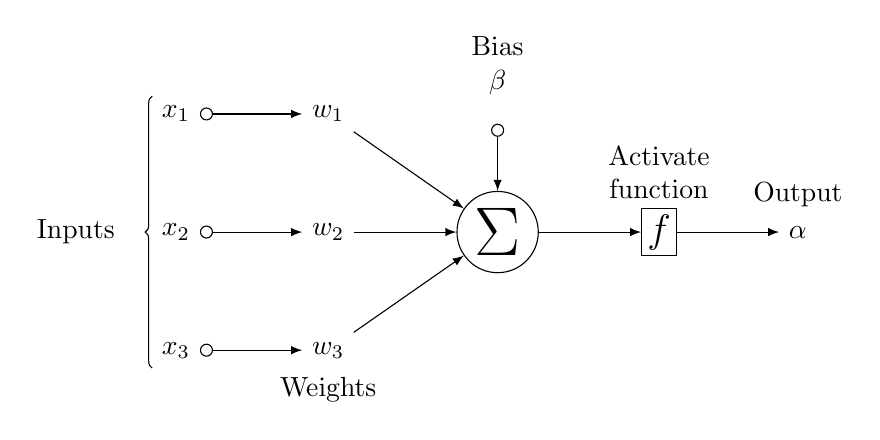
\begin{tikzpicture}[
    init/.style={
      draw,
      circle,
      inner sep=2pt,
      font=\Huge,
      join = by -latex
    },
    squa/.style={
      draw,
      inner sep=2pt,
      font=\Large,
      join = by -latex
    },
    start chain=2,node distance=13mm
    ]
    \node[on chain=2] 
      (x2) {$x_2$};
    \node[on chain=2,join=by o-latex] 
      {$w_2$};
    \node[on chain=2,init] (sigma) 
      {$\displaystyle\Sigma$};
    \node[on chain=2,squa,label=above:{\parbox{2cm}{\centering Activate \\ function}}]   
      {$f$};
    \node[on chain=2,label=above:Output,join=by -latex] 
      {$\alpha$};
    \begin{scope}[start chain=1]
    \node[on chain=1] at (0,1.5cm) 
      (x1) {$x_1$};
    \node[on chain=1,join=by o-latex] 
      (w1) {$w_1$};
    \end{scope}
    \begin{scope}[start chain=3]
    \node[on chain=3] at (0,-1.5cm) 
      (x3) {$x_3$};
    \node[on chain=3,label=below:Weights,join=by o-latex] 
      (w3) {$w_3$};
    \end{scope}
    \node[label=above:\parbox{2cm}{\centering Bias \\ $\beta$}] at (sigma|-w1) (b) {};
    
    \draw[-latex] (w1) -- (sigma);
    \draw[-latex] (w3) -- (sigma);
    \draw[o-latex] (b) -- (sigma);
    
    \draw[decorate,decoration={brace,mirror}] (x1.north west) -- node[left=10pt] {Inputs} (x3.south west);
\end{tikzpicture}
\textit{An example node in a neural network}


\section{Activation Functions}
The activation function is a non-linear function that is applied to the output of a node.

\subsection{Sigmoid}
Sigmoid is a commonly used activation function, as it is simple and smooth.
It allows for the network to learn complex patterns in the data, as it is non-linear.
The function is as follows:
\begin{equation}
    \sigma(x) = \frac{1}{1+e^{-x}}
\end{equation}

The sigmoid function however can suffer from the vanishing gradient problem, where the gradient of the function becomes very small as the input becomes very large.
This can lead to the network not learning as well, as the weights are not updated as much.

\subsection{Tanh}
The tanh function is similar to the sigmoid function, but is centred around 0, with a range of -1 to 1.
The function is as follows:
\begin{equation}
    \tanh(x) = \frac{e^{x} - e^{-x}}{e^{x} + e^{-x}}
\end{equation}

The tanh function also suffers from vanishing gradients, as it has a similar structure to sigmoid, however its range is from -1 to 1, so it is more useful for normalising the data.

\subsection{ReLU}
The ReLU (Rectified Linear Unit) function is a simple function that is used in many neural networks.
It is a piecewise function, with the function being 0 for all negative values, and the input for all positive values.
The function is as follows:
\begin{equation}
    f(x) = \max(0, x)
\end{equation}

The ReLU function is used as it is simple and computationally efficient, and it does not suffer from the vanishing gradient problem.
However, it can suffer from the dying ReLU problem, where the gradient of the function is 0 for all negative values, and the weights are not updated.



\section{Cost Functions}

There are 2 main loss functions that can be used in a neural network, the mean squared error (MSE) and the mean absolute error (MAE). 
The MSE is the most common loss function used in neural networks, as it is differentiable and convex.
The MAE is less common, but is more robust to outliers in the data.
\vspace{1em}
\newline
We use the cost function to calculated the error of the network, and then use the gradient of the cost function to adjust the weights of the network.
\subsection{Mean Squared Error}
The MSE equation is as follows:
\begin{equation}
    \text{MSE} = \frac{1}{n}\sum_{i=1}^{n}(E_m - O_m)^2
\end{equation}
Where $E_m$ is the expected output and $O_m$ is the actual output.

We differentiate this with respect to output $O_m$ to get the gradient of the cost function.
\begin{equation}
    \frac{\partial \text{MSE}}{\partial O_m} = \frac{-2}{n}(E_m - O_m)
\end{equation}

For large datasets, this can make the error of the network small and meaningless, leading to large training times.

\subsection{Mean Absolute Error}
The MAE equation is as follows:
\begin{equation}
    \text{MAE} = \frac{1}{n}\sum_{i=1}^{n}|E_m - O_m|
\end{equation}

We differentiate this with respect to output $O_m$ to get the gradient of the cost function.

\begin{equation}
    \frac{\partial \text{MAE}}{\partial O_m} = \frac{1}{n}\sum_{i=1}^{n}\frac{E_m - O_m}{|E_m - O_m|}
\end{equation}
This gives us the following results for each case:
\begin{equation}
\frac{\partial MAE}{\partial O_m} =
\begin{cases} 
\frac{1}{n}, & \text{if } O_m > E_m \\ 
-\frac{1}{n}, & \text{if } O_m < E_m 
\end{cases}
\end{equation}
As you cannot divide by 0, there is not a smooth gradient at $O_m = E_m$.

Another potential issue is that as the gradient does not rely on the output, the network may not learn as well as with the MSE.
This however is its strength, as it is more robust to outliers in the data, as it won't skew the data as much as the MSE.
\vspace{1em}
\newline
For this project, I will use the MSE as the loss function, as the data has been cleaned and interpolated, and the outliers have been removed.
However, I will use a variation of the MSE.

The function I will use is:

\begin{equation}
    \frac{\delta MSE}{\delta O_m}  = C(E_m, O_m) = E_m - O_m
\end{equation}
This is because the gradient is dependent on the output, and the network will learn better with this function.
It also removes the negative gradient as a negative gradient pushes the network in the wrong direction with my implementation of the back propagation algorithm.
I have also removed the division by $n$ as it will stifle my learning rate, as the data is already normalised and $n$ is a constant.

\section{Forward Pass}

For $n$ inputs, $m$ hidden nodes in layer $\mathcal{L}$ and $q$ output nodes.
\vspace{1em}
\newline
The input matrix takes the $n$ data points from the training data in the form:
\begin{equation}
    \text{Matrix }\mathbf{I}\rightarrow \left[1\times n\right] : \mathbf{I} = 
        \begin{vmatrix}
        \mathbf{I}_1 ,& \mathbf{I}_2 ,&\cdots, & \mathbf{I}_n
        \end{vmatrix}
\end{equation}
\newline
The weight matrix $\omega^1$ is a $n\times m$ matrix, with each row representing the weights of a input nodes to each connected hidden node in the first hidden layer.
\begin{equation}
    \text{Matrix }\omega^{1}\rightarrow \left[n\times m\right] : \omega^1 = 
        \begin{vmatrix}
        \omega_{11}^{1} ,& \omega_{12}^{1} ,&\cdots, & \omega_{1m}^{1} \\
        \omega_{21}^{1} ,& \ddots & & \omega_{2m}^{1} \\
        \vdots  & &\ddots & \vdots  \\
        \omega_{n1}^{1} ,& \omega_{n2}^{1} ,&\cdots, & \omega_{nm}^{1} \\
        \end{vmatrix}
\end{equation}
\newline
The matrix multiplication of the input matrix and the weight matrix gives us a matrix of dimensions $1\times m$.
This correlates to the amount of nodes in the first hidden layer, a sum of weights multiplied by their corresponding input data for each hidden node.
\begin{equation}
    \text{Matrix }\mathbf{I}\cdot\omega^{1}\rightarrow \left[1\times n\right]\cdot\left[n\times m\right]\rightarrow \left[1\times m\right]: \mathbf{I}\cdot\omega =
        \begin{vmatrix}
        \mathbf{I}_1\cdot\omega_{11}^{1} + \cdots +  \mathbf{I}_n\cdot\omega_{n1}^{1} ,& \cdots, \mathbf{I}_m\cdot\omega_{1m}^{1} + \cdots +  \mathbf{I}_n\cdot\omega_{nm}^{1}
        \end{vmatrix}
\end{equation}
\newline
Each node in the hidden layer will have a bias term $\beta$.
Formatting this as a matrix, we get a $1\times m$ matrix, which aligns with the dimensions matrix $\mathbf{I}\cdot\omega$ (2.5.3).
\begin{equation}
    \text{Matrix }\beta^{1}\rightarrow \left[1\times m\right] : \beta^{1}  = 
        \begin{vmatrix}
            \beta_{1}^{1} ,& \beta_{2}^{1} ,&\cdots, & \beta_{m}^{1}
        \end{vmatrix}
\end{equation}
\newline
We apply an element-wise summation of the matrix $\mathbf{I}\cdot\omega$ and the bias matrix $\beta$, to find the matrix $\mathcal{S}^1\rightarrow \left[1\times m \right]$: the summation of each node in layer 1.
Applying the activation function $\mathcal{F}_1$ to the summation matrix $\mathcal{S}$ gives us the output $\alpha$ of the hidden layer.

\textit{Note that the activation function is labeled $\mathcal{F}_1$ as it is the first activation function in the network, and can differ from other activation functions in the network.}
\begin{align}
    \text{Matrix }\alpha\rightarrow \left[1\times m\right] : \alpha  = 
    \mathcal{F}_1(\mathcal{S}^{1}) &= \mathcal{F}_1(\mathbf{I}\cdot\omega^{1} + \beta^{1})\\
    \text{where }\mathcal{S}^1_m &= \sum_{k=1}^{n} \Big(\mathbf{I}_k\cdot\omega_{km}^{1}\Big) + \beta_{m}^{1}
\end{align}
This activation function is applied to every element in the matrix.
This matrix $\alpha$ is then used as the input for the next hidden layer of the network, repeating the same process as before all the way to the output layer:
\newline
The weight matrix $\omega^{\mathcal{L}}$ is a $n\times m$ matrix, with each row representing the weights of a hidden node ($n$) in layer $\mathcal{L}-1$ to each connected node($m$) in layer $\mathcal{L}$.
\begin{align}
    \text{Matrix }\omega^{\mathcal{L}}\rightarrow \left[n\times m\right] : \omega^{\mathcal{L}} &= 
        \begin{vmatrix}
        \omega_{11}^{\mathcal{L}} ,& \omega_{12}^{\mathcal{L}} ,&\cdots, & \omega_{1m}^{\mathcal{L}} \\
        \omega_{21}^{\mathcal{L}} ,& \ddots & & \omega_{2m}^{\mathcal{L}} \\
        \vdots  & &\ddots & \vdots  \\
        \omega_{n1}^{\mathcal{L}} ,& \omega_{n2}^{\mathcal{L}} ,&\cdots, & \omega_{nm}^{\mathcal{L}} \\
        \end{vmatrix}\\
        \\
        \text{Matrix }\beta^{\mathcal{L}}\rightarrow \left[1\times m\right] : \beta^{\mathcal{L}}  &= 
        \begin{vmatrix}
            \beta_{1}^{\mathcal{L}} \hspace{4pt},& \beta_{2}^{\mathcal{L}}\hspace{4pt} ,&\cdots, & \beta_{m}^{\mathcal{L}\hspace{4pt}}
        \end{vmatrix}
\end{align}
for $l$ hidden layers.
\vspace{1em}
\newline
The same summation applies to the hidden layer output $\alpha$ and the weight matrix $\omega$ for each hidden layer, all the way to the output layer.
We travel layer by layer to reach our predicted output, $\mathcal{O}_{q}$.

\begin{align}
    \text{Matrix }\alpha^{\mathcal{L}}\rightarrow \left[1\times m\right] : \alpha^{\mathcal{L}}  = 
    \mathcal{F}_\mathcal{L}(\mathcal{S}^{\mathcal{L}}) &= \mathcal{F}_{\mathcal{L}}\Big(\alpha^{\mathcal{L}-1}\cdot\omega^{\mathcal{L}} + \beta^{\mathcal{L}}\Big)\\
    \text{where }\mathcal{S}^{\mathcal{L}}_{m} &= \sum_{k=1}^{n} \Big( \alpha_k^{\mathcal{L}-1}\cdot\omega^{\mathcal{L}}_{km} \Big) + \beta^{\mathcal{L}}_{m}
\end{align}
\textit{Note that $\mathcal{F}_\mathcal{L}$ is the activation function at layer $\mathcal{L}$.}
\newline
\vspace{1em}
Finally, we calculate the output of the network, $\mathcal{O}_{q}$.
\begin{equation}
    \text{Output }\rightarrow \left[1\times q\right] : \mathcal{O}_{q}  = 
    \mathcal{F}_\mathcal{L}(\mathcal{S}^{\mathcal{L}}) = \mathcal{F}_\mathcal{L}(\alpha^{\mathcal{L}-1}\cdot\omega^{\mathcal{L}} + \beta^{\mathcal{L}})
\end{equation}
This gives us our prediction from the forward pass through the network. 
\vspace{1em}
\newline
An example of a network with 1 hidden node is given below:
\vspace{1em}
\newline
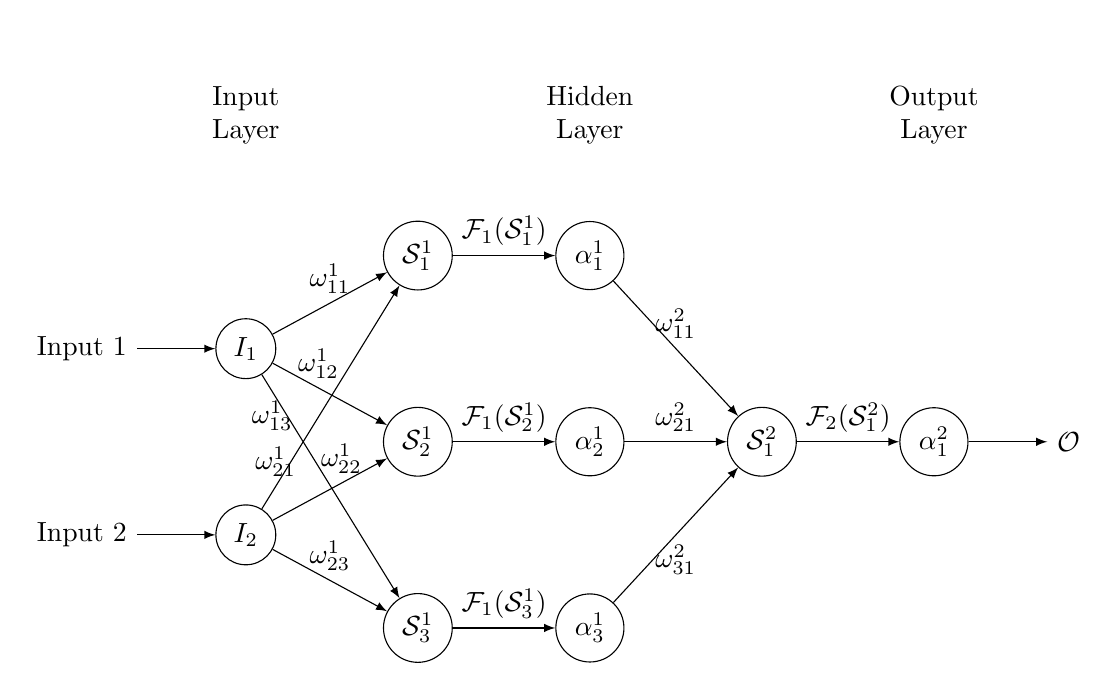
\begin{tikzpicture}[
    net/.style={
      matrix of nodes,
      nodes={draw, circle, minimum size=0.75cm},
      column sep=0.75cm,
      row sep=10pt
    },
    >=latex
]

  % Define the matrix
  \matrix[net] (mat) {
    |[draw=none]| \parbox{1.5cm}{\centering Input\\Layer} & &|[draw=none]| \parbox{1.5cm}{\centering Hidden\\Layer} & &|[draw=none]| \parbox{1.5cm}{\centering Output\\Layer} \\
    & $\mathcal{S}_{1}^1$  & $\alpha_{1}^1$ \\
    $I_1$ & \\
    & $\mathcal{S}_{2}^1$  & $\alpha_{2}^1$ & $\mathcal{S}_{1}^2$  & $\alpha_{1}^2$\\
    $I_2$ & \\
    & $\mathcal{S}_{3}^1$  & $\alpha_{3}^1$ \\
  };

  % input labels
  \foreach \i [count=\j] in {3,5}
  \draw[<-] (mat-\i-1.west) -- ++(-1cm,0) node[left] {Input \j};

  % Connections from input to hidden layer 1
    \draw[->] (mat-3-1) -- (mat-2-2) node[midway, above] {$\omega^{1}_{11}$};
    \draw[->] (mat-3-1) -- (mat-4-2) node[pos=0.4, above] {$\omega^{1}_{12}$};
    \draw[->] (mat-3-1) -- (mat-6-2) node[pos=0.075, below] {$\omega^{1}_{13}$};
    \draw[->] (mat-5-1) -- (mat-2-2) node[pos=0.1, above] {$\omega^{1}_{21}$};
    \draw[->] (mat-5-1) -- (mat-4-2) node[pos=0.6, above] {$\omega^{1}_{22}$};
    \draw[->] (mat-5-1) -- (mat-6-2) node[midway, above] {$\omega^{1}_{23}$};

    % Connections from hidden layer 1 to hidden layer 1
    \draw[->] (mat-2-2) -- (mat-2-3) node[midway, above] {$\mathcal{F}_1(\mathcal{S}_{1}^1)$};
    \draw[->] (mat-4-2) -- (mat-4-3) node[midway, above] {$\mathcal{F}_1(\mathcal{S}_{2}^1)$};
    \draw[->] (mat-6-2) -- (mat-6-3) node[midway, above] {$\mathcal{F}_1(\mathcal{S}_{3}^1)$};

    % Connections from hidden layer 1 to output layer
    \draw[->] (mat-2-3) -- (mat-4-4) node[midway, above] {$\omega^{2}_{11}$};
    \draw[->] (mat-4-3) -- (mat-4-4) node[midway, above] {$\omega^{2}_{21}$};
    \draw[->] (mat-6-3) -- (mat-4-4) node[midway, below] {$\omega^{2}_{31}$};

    \draw[->] (mat-4-4) -- (mat-4-5) node[midway, above] {$\mathcal{F}_2(\mathcal{S}_{1}^2)$};


    % output labels
    \foreach \i [count=\j] in {4}
    \draw[->] (mat-\i-5.east) -- ++(1cm,0) node[right] {$\mathcal{O}$};



\end{tikzpicture}
\textit{$I=2, m=3, q=1, l=1$}

\section{Backward Pass}
The backward pass is used to update the weights and biases of the network, to reduce the error of the network and improve the accuracy of the model.
Back propagation is about finding how much of the error is due to each weight in the network, and then updating the weights to reduce the error.
\vspace{1em}
\newline
Leibniz's notation of the chain rule is used to find the partial derivative of the error with respect to the weights and biases in the network.
Leibniz's notation states that \textit{If a variable z depends on the variable y, which itself depends on the variable x (that is, y and z are dependent variables), then z depends on x as well, via the intermediate variable y.}
\begin{align}
    \frac{\delta z}{\delta x} = \frac{\delta z}{\delta y}\cdot\frac{\delta y}{\delta x}
\end{align}
\vspace{1em}
\newline
To back propagate through the network, we need to find how much of the error (cost $C$) is due to each node in the network so that we can update the weights and biases to reduce the cost for future predictions.
Using the chain rule, we can find the rate of change of the error with respect to the weights and biases in the network, working backwards from the output to each node.
We can use partial derivatives to find the rate of change of the error with respect to each weight and bias in the network, by differentiating the weights and biases dependent variables.
\begin{equation}
    \frac{\delta C}{\delta \omega^{\mathcal{L}}_{nm}} = \frac{\delta C}{\delta \mathcal{S}^{\mathcal{L}}_m}\cdot\frac{\delta \mathcal{S}^{\mathcal{L}}_m}{\delta \omega^{\mathcal{L}}_{nm}} \hspace{30pt}
    \frac{\delta C}{\delta \beta^{\mathcal{L}}_{nm}} = \frac{\delta C}{\delta \mathcal{S}^{\mathcal{L}}_m}\cdot\frac{\delta \mathcal{S}^{\mathcal{L}}_m}{\delta \beta^{\mathcal{L}}_{nm}}
\end{equation}
Using the equation for $\mathcal{S}$ that we found in (2.5.11), we can differentiate the summation with respect to the weights and biases in the network:
\begin{align}
    \mathcal{S}^{\mathcal{L}}_{m} &= \sum_{k=1}^{n} \Big( \alpha_k^{\mathcal{L}-1}\cdot\omega^{\mathcal{L}}_{km} \Big) + \beta^{\mathcal{L}}_{m} &\rightarrow
    \frac{\delta}{\delta \omega^{\mathcal{L}}_{nm}} \sum_{k=1}^{n} \Big( \alpha_k^{\mathcal{L}-1}\cdot\omega^{\mathcal{L}}_{km} \Big) &+ \beta^{\mathcal{L}}_{m} &=
    \alpha_{n}^{\mathcal{L}-1}\\
    \mathcal{S}^{\mathcal{L}}_{m} &= \sum_{k=1}^{n} \Big( \alpha_k^{\mathcal{L}-1}\cdot\omega^{\mathcal{L}}_{km} \Big) + \beta^{\mathcal{L}}_{m} &\rightarrow
    \frac{\delta}{\delta \beta ^{\mathcal{L}}_{m}} \sum_{k=1}^{n} \Big( \alpha_k^{\mathcal{L}-1}\cdot\omega^{\mathcal{L}}_{km} \Big) &+ \beta^{\mathcal{L}}_{m} &= 1
\end{align}
Substituting into (2.6.2):
\begin{align}
    \frac{\delta C}{\delta \omega^{\mathcal{L}}_{nm}} &=  \alpha_{n}^{\mathcal{L}-1} \cdot\frac{\delta C}{\delta \mathcal{S}^{\mathcal{L}}_m}  &\rightarrow& \hspace{10pt}\alpha_{n}^{\mathcal{L}-1} \cdot\frac{\delta C}{\delta \alpha^{\mathcal{L}}_m}\cdot\frac{\delta \alpha^{\mathcal{L}}_m}{\delta \mathcal{S}^{\mathcal{L}}_m} \\
    \frac{\delta C}{\delta \beta^{\mathcal{L}}_{m}} &= 1 \cdot\frac{\delta C}{\delta \mathcal{S}^{\mathcal{L}}_m} &\rightarrow& \hspace{10pt}1 \cdot\frac{\delta C}{\delta \alpha^{\mathcal{L}}_m}\cdot\frac{\delta \alpha^{\mathcal{L}}_m}{\delta \mathcal{S}^{\mathcal{L}}_m}\qquad \qquad \qquad \qquad \qquad \qquad \qquad
\end{align}
Then it follows with equation (2.5.10):
\begin{align}
    \frac{\delta \alpha^{\mathcal{L}}_m}{\delta \mathcal{S}^{\mathcal{L}}_m} = \mathcal{F}'_{\mathcal{L}}(\mathcal{S}^{\mathcal{L}}_m)\hspace{30pt}\rightarrow&  \frac{\delta C}{\delta \omega^{\mathcal{L}}_{nm}} = \alpha_{n}^{\mathcal{L}-1} \cdot \mathcal{F}'_{\mathcal{L}}(\mathcal{S}^{\mathcal{L}}_m) \cdot \frac{\delta C}{\delta \alpha^{\mathcal{L}}_m}\\
    \rightarrow& \frac{\delta C}{\delta \beta^{\mathcal{L}}_{m}} = \mathcal{F}'_{\mathcal{L}}(\mathcal{S}^{\mathcal{L}}_m) \cdot \frac{\delta C}{\delta \alpha^{\mathcal{L}}_m}
\end{align}
As we are moving backwards through the network, we use the same theory that the gradient at the node is the sum of the gradients of the weights it is connected to,
Where are influenced by the gradient at the node it is connected to. We call this value $\delta$.
\begin{align}
    \frac{\delta C}{\delta \alpha^{\mathcal{L}}_m} = \sum_{p=1}^{q}\Big(\frac{\delta C}{\delta \omega^{\mathcal{L}+1}_{mp}}\Big) = \sum_{p=1}^{q}\Big(\delta^{\mathcal{L}+1}_{p} \cdot \omega^{\mathcal{L}+1}_{mp}\Big)
\end{align}
Referencing to our example network:
\vspace{1em}
\newline
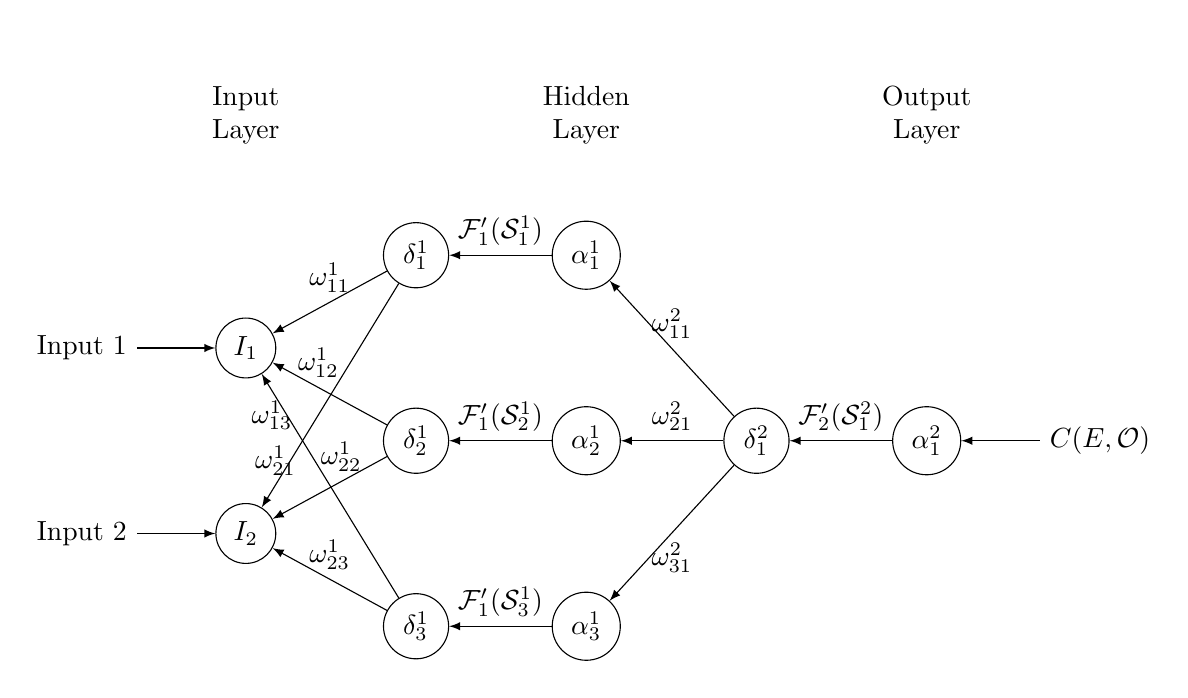
\begin{tikzpicture}[
    net/.style={
      matrix of nodes,
      nodes={draw, circle, minimum size=0.75cm},
      column sep=0.75cm,
      row sep=10pt
    },
    >=latex
]

  % Define the matrix
  \matrix[net] (mat) {
    |[draw=none]| \parbox{1.5cm}{\centering Input\\Layer} & &|[draw=none]| \parbox{1.5cm}{\centering Hidden\\Layer} & &|[draw=none]| \parbox{1.5cm}{\centering Output\\Layer} \\
    & $\delta_{1}^1$  & $\alpha_{1}^1$ \\
    $I_1$ & \\
    & $\delta_{2}^1$  & $\alpha_{2}^1$ & $\delta_{1}^2$  & $\alpha_{1}^2$\\
    $I_2$ & \\
    & $\delta_{3}^1$  & $\alpha_{3}^1$ \\
  };

  % input labels
  \foreach \i [count=\j] in {3,5}
  \draw[<-] (mat-\i-1.west) -- ++(-1cm,0) node[left] {Input \j};

  % Connections from input to hidden layer 1
    \draw[<-] (mat-3-1) -- (mat-2-2) node[midway, above] {$\omega^{1}_{11}$};
    \draw[<-] (mat-3-1) -- (mat-4-2) node[pos=0.4, above] {$\omega^{1}_{12}$};
    \draw[<-] (mat-3-1) -- (mat-6-2) node[pos=0.075, below] {$\omega^{1}_{13}$};
    \draw[<-] (mat-5-1) -- (mat-2-2) node[pos=0.1, above] {$\omega^{1}_{21}$};
    \draw[<-] (mat-5-1) -- (mat-4-2) node[pos=0.6, above] {$\omega^{1}_{22}$};
    \draw[<-] (mat-5-1) -- (mat-6-2) node[midway, above] {$\omega^{1}_{23}$};

    % Connections from hidden layer 1 to hidden layer 1
    \draw[<-] (mat-2-2) -- (mat-2-3) node[midway, above] {$\mathcal{F}'_1(\mathcal{S}_{1}^1)$};
    \draw[<-] (mat-4-2) -- (mat-4-3) node[midway, above] {$\mathcal{F}'_1(\mathcal{S}_{2}^1)$};
    \draw[<-] (mat-6-2) -- (mat-6-3) node[midway, above] {$\mathcal{F}'_1(\mathcal{S}_{3}^1)$};

    % Connections from hidden layer 1 to output layer
    \draw[<-] (mat-2-3) -- (mat-4-4) node[midway, above] {$\omega^{2}_{11}$};
    \draw[<-] (mat-4-3) -- (mat-4-4) node[midway, above] {$\omega^{2}_{21}$};
    \draw[<-] (mat-6-3) -- (mat-4-4) node[midway, below] {$\omega^{2}_{31}$};

    \draw[<-] (mat-4-4) -- (mat-4-5) node[midway, above] {$\mathcal{F}'_2(\mathcal{S}_{1}^2)$};


    % output labels
    \foreach \i [count=\j] in {4}
    \draw[<-] (mat-\i-5.east) -- ++(1cm,0) node[right] {$C(E,\mathcal{O})$};



\end{tikzpicture}
\textit{$I=2, m=3, q=1, l=1$}
This sum is the result of propagating error back through the network and is the backbone of the back propagation algorithm.
Finally substituting this back into (2.6.7) and (2.6.8) we get the following:
\begin{align}
    \frac{\delta C}{\delta \omega^{\mathcal{L}}_{nm}} &= \alpha_{n}^{\mathcal{L}-1} \cdot \mathcal{F}'_{\mathcal{L}}(\mathcal{S}^{\mathcal{L}}_m) \cdot \sum_{p=1}^{q}\Big(\delta^{\mathcal{L}+1}_{p} \cdot \omega^{\mathcal{L}+1}_{mp}\Big)\\
    \frac{\delta C}{\delta \beta^{\mathcal{L}}_{m}} &= \mathcal{F}'_{\mathcal{L}}(\mathcal{S}^{\mathcal{L}}_m)\cdot\sum_{p=1}^{q}\Big(\delta^{\mathcal{L}+1}_{p} \cdot \omega^{\mathcal{L}+1}_{mp}\Big)
\end{align}
\vspace{1em}
\newline
Using what we derived, we can find a formula for the delta values of the nodes in the network, collecting like terms from the equations above(2.6.10), (2.6.11).
\begin{align}
    \frac{\delta C}{\delta \omega^{\mathcal{L}}_{nm}} &= \alpha_{n}^{\mathcal{L}-1} \cdot \delta^{\mathcal{L}}_{m}\\
    \frac{\delta C}{\delta \beta^{\mathcal{L}}_{m}} &= \delta^{\mathcal{L}}_{m}
\end{align}
\vspace{1em}
\newline
These delta values can be used in the form of matrices in our network to update the weights and biases.
For the output layer, the delta value is the output of the cost function derivative, as 100\% of the error comes through the output layer, and then we apply the derivative of the activation function.
\begin{align}
    \delta^{\mathcal{L}}_{m} &= C(E_{m},O_{m})\cdot\mathcal{F}'_{m}(\mathcal{S}^{\mathcal{L}}_{m}) \notag\\
    \text{Matrix }\delta^{\mathcal{L}}_{m} \rightarrow \left[1 \times m\right]:  \delta^{\mathcal{L}}_{m} &=
    \begin{vmatrix}
        C(E_{1},O_{1})\cdot\mathcal{F}'_{1}(\mathcal{S}^{\mathcal{L}}_{1}), & \cdots, & C(E_{m},O_{m})\cdot\mathcal{F}'_{m}(\mathcal{S}^{\mathcal{L}}_{m})
    \end{vmatrix} 
\end{align}
Where $C(C_{m},\mathcal{O}_{m})$ is the cost function derivative, $E_{m}$ is the expected output and $O_{m}$ is the predicted output of the node.
\vspace{1em}
\newline
We can then construct an equation for the delta values of the hidden nodes in the network.

\textit{For the hidden nodes in layers $1\leq k < \mathcal{L}$:}
\begin{align}
    \delta^{k}_{n} = \mathcal{F}'_{k}(\mathcal{S}^{k}_n)\cdot&\sum_{p=1}^{q}\Big(\delta^{k+1}_{p} \cdot \omega^{k+1}_{np}\Big) \notag\\
    &\sum_{p=1}^{q}\Big(\delta^{k+1}_{p} \cdot \omega^{k+1}_{np}\Big) \rightarrow \text{ Matrix } \left[1 \times p\right] \cdot \left[n \times p\right]^{T} \rightarrow \left[1 \times n\right]\notag\\
    \text{Matrix }\delta^{k}_{n} \rightarrow \left[1 \times n\right] \circ \left[1 \times n\right]  \rightarrow \left[1 \times n\right] :  \delta^{k}_{n} =&
    \begin{vmatrix}
        \mathcal{F}'_{k}(\mathcal{S}^{k}_1)\cdot\sum_{p=1}^{q}\Big(\delta^{k+1}_{p} \cdot \omega^{k+1}_{1p}\Big), \cdots,\mathcal{F}'_{k}(\mathcal{S}^{k}_n)\cdot\sum_{p=1}^{q}\Big(\delta^{k+1}_{p} \cdot \omega^{k+1}_{np}\Big)
    \end{vmatrix}
\end{align}
With $n$ nodes in layer $k$, $p$ nodes in layer $k+1$ and $\omega_{nq}^{k+1}$ being the weight between node $n$ in layer $k$ and node $q$ in layer $k+1$.
With $\circ$ being the element-wise multiplication of the two matrices.
\vspace{1em}
\newline
Using our findings from equation (2.6.10) and (2.6.11), we can update the weights and biases in the network.
We can update the weights and biases in the network by adding the gradient, multiplied by the learning rate $\eta$.  
This decides how much of the gradient we want to apply to the weights and biases for our next forward pass.

% add matrix calculations to the weights and biases %
% calculate all the deltas friest then calcualte weights and biases %
%update to show that???%
\begin{equation}
    \text{Matrix }\omega^{k}_{nq}\rightarrow\left[n \times q\right] + \left[1 \times n\right]^T \cdot \left[1 \times q\right]  \rightarrow \left[n \times q\right] :\omega'^{k}_{nq} = \omega^{k}_{nq} + \eta\cdot\alpha_{n}^{k-1}\cdot\delta^{k}_{q}
\end{equation}

\begin{equation}
    \text{Matrix }\beta'^{k}_{nq}\rightarrow \left[n \times q\right] + \left[1 \times q\right]  \rightarrow \left[n \times 1\right] :\beta'^{k}_{nq} = \beta^{k}_{nq} + \eta\cdot\delta^{k}_{q}
\end{equation}
It is worth remembering that we only update the weights and biases after we have calculated all the delta values for the network, as the error of the network is dependent on what these values were when the forward pass was made.
Once we calculate the delta values for the network, we can then update the weights and biases.


\section{Implementation of a single hidden layer network}

A single hidden layer can be implemented with a defined structure.
As we know how many nodes and layers there are, we can hard code the dimensions. 
We can initialise the weights and biases randomly, with the structure that we define.

\begin{lstlisting}[language=Python]
back_prop_single.py

    import numpy as np

    # Define the structure of the network
    perceptronStructure = (7, 16, 1)

    def init_structure(perceptronStructure):
        '''Intialises the perceptron structure with random weights'''

        # Weights and biases for input layer to the hidden layer
        hiddenWeightMatrix = np.random.uniform(-1, 1, (perceptronStructure[0], perceptronStructure[1]))
        hiddenBiasMatrix = np.random.uniform(-1, 1, (1, perceptronStructure[1]))

        # Weights and biases for hidden layer to the output layer
        outputWeightMatrix = np.random.uniform(-1, 1, (perceptronStructure[1], perceptronStructure[2]))
        outputBiasMatrix = np.random.uniform(-1, 1, (1, perceptronStructure[2]))

        # Create lists for input and output
        hiddenList = [hiddenWeightMatrix, hiddenBiasMatrix]
        outputList = [outputWeightMatrix, outputBiasMatrix]

        return hiddenList, outputList


    hiddenList, outputList = init_structure(perceptronStructure)

\end{lstlisting}
In this example, we have a network with 7 input nodes, 16 hidden nodes and 1 output node.
\vspace{1em}
\newline
We iterate through each of the data points and pass them through the forward pass of the network.
We pass them through a scaling function to normalise the data, then pass them through the network.
By doing this, the network can appropriately learn to predict the output as all datapoints are are passed through an activation function that outputs between 0 and 1.
\begin{lstlisting}[language=Python]
back_prop_single.py

    # Normalization function
    def min_max_scaler(data):
        '''Function to normalize the data'''
        return (data - data.min()) / (data.max() - data.min())

    def min_max_reverser(data, dataMax, dataMin):
        '''Function to normalize the data'''
        return data * (dataMax - dataMin) + dataMin


    def forward_pass(data, hiddenList, outputList):
        '''Forward pass of the neural network'''

        # Calculate for the hidden layer
        hiddenSum = (inputData @ hiddenList[0]) + hiddenList[1]
        hiddenActivated = sigmoid(hiddenSum)

        # Calculate for the output layer
        outputSum = (hiddenActivated @ outputList[0]) + outputList[1]
        outputActivated = sigmoid(outputSum)

        return hiddenSum, hiddenActivated, outputSum, outputActivated


    while count < epochs:

        # Iterate through the training data
        for i, day in enumerate(trainingData.itertuples(index=False), start=0):

            inputData = np.array([float(day[2]), float(day[3]), float(day[4]), float(day[5]), float(day[6]), float(day[7]), float(day[8])])
            expectedOutput = np.array([float(day[1])])

            # Forward pass
            hiddenSum, hiddenActivated, outputSum, outputActivated = forward_pass(inputData, hiddenList, outputList)

\end{lstlisting}

\vspace{1em}
We can then expand by introducing the backward pass to update the weights and biases of the network.

\begin{lstlisting}[language=Python]
back_prop_single.py

    def backward_pass(expectedOutput, hiddenSum, hiddenActivated, outputSum, outputActivated, hiddenList, outputList, inputData, dfLength):
        '''Backward pass of the neural network'''

        # Calculate the cost of the perceptron structure
        structureCost = cost_function_derivative(expectedOutput, outputActivated, dfLength)

        # Calculate the delta values for the output layer
        outputDelta = structureCost * sigmoid_derivative(outputSum)

        # Calculate the delta values for the hidden layer
        hiddenDelta = (outputDelta @ outputList[0].T) * sigmoid_derivative(hiddenSum)


        # Update the weights and biases for the output layer
        outputList[0] += (hiddenActivated.T @ outputDelta) * learningRate
        outputList[1] += outputDelta * learningRate

        # Update the weights and biases for the hidden layer
        hiddenList[0] += (inputData.T @ hiddenDelta) * learningRate
        hiddenList[1] += hiddenDelta * learningRate

        return (hiddenList, outputList)


    while count < epochs:

        # Iterate through the training data
        for i, day in enumerate(trainingData.itertuples(index=False), start=0):

            inputData = np.array([float(day[2]), float(day[3]), float(day[4]), float(day[5]), float(day[6]), float(day[7]), float(day[8])])
            expectedOutput = np.array([float(day[1])])

            # Forward pass
            hiddenSum, hiddenActivated, outputSum, outputActivated = forward_pass(inputData, hiddenList, outputList)
            hiddenList, outputList = backward_pass(expectedOutput, hiddenSum, hiddenActivated, outputSum, outputActivated, hiddenList, outputList, inputData.reshape(1, -1), dfLength)

        count += 1


\end{lstlisting}

We can then create predictions after a given amount of epochs, and calculate the error of the network.
We can then plot these predictions against the expected output to see how well the network is performing.
\vspace{1em}
\newline
A single layer network does not allow for complex patterns to be learned, so to improve the network, we can add more hidden layers to the network.
As stated previously, repeatedly using the sigmoid activation over multiple layers can cause the gradient to vanish, so we can allow the activation to be defined for each indeviual layer.


\section{Multiple Hidden Layers}
To implement multiple hidden layers, we can define the structure of the network as a tuple.
The first element of the tuple is the number of input nodes, and the second element is a list of tuples, each with the amount of nodes and their activation function.
We can iteratively generate hidden layers and then use the same process to calculate changes and weight updates.

\begin{lstlisting}[language=Python]
back_prop_multi.py

    import numpy as np

    # Define the structure of the network
    perceptronStructure = (7, [(16, 'sigmoid'),(16, 'sigmoid'), (1, 'sigmoid')])

    # Initialise Perceptron Structure
    def init_structure(perceptronStructure):
        '''Initialises the perceptron structure'''

        # Split structure
        inputDimensions = perceptronStructure[0]
        nodeDimensions = perceptronStructure[1]

        # Create lists for weights and biases
        weightList = []
        biasList = []

        # Initialise the first layer of the perceptron
        weightMatrix = np.random.uniform(-1, 1, (inputDimensions, nodeDimensions[0][0]))
        biasMatrix = np.random.uniform(-1, 1, (1, nodeDimensions[0][0]))

        # Append to the lists
        weightList.append(weightMatrix)
        biasList.append(biasMatrix)

        # Initialise the node layers of the perceptron
        for i in range(1, len(nodeDimensions)):
            weightMatrix = np.random.uniform(-1, 1, (nodeDimensions[i - 1][0], nodeDimensions[i][0]))
            biasMatrix = np.random.uniform(-1, 1, (1, nodeDimensions[i][0]))

            # Append to the lists
            weightList.append(weightMatrix)
            biasList.append(biasMatrix)

        return weightList, biasList


\end{lstlisting}
As each layer can have its own activation function, we can define the activation function for each layer.
To do this, each layer has a tuple with the number of nodes and the activation function.
These are then stored as a list and joined with the input dimensions to create the structure of the network.
\vspace{1em}
\newline
The structure we use to iterate through the layers is the same as our backwards pass.
We calculate our first item, and then iterate through the rest of the layers until we reach the end.

However, for the forward pass, we just go through the whole list and calculate the forward pass for each layer iteratively.
This is because it is simpler and each step is the same computation
\begin{lstlisting}[language=Python]
back_prop_multi.py
    
    import numpy as np

    layerStructure = perceptronStructure[1]

    def forward_pass(inputData, weightList, biasList, layerStructure):
        '''Forward pass of the neural network'''

        # Create a list for the activated nodes and summed nodes
        summedList = []
        activatedList = []


        # Calculate for the hidden layers
        for layer, structure in enumerate(layerStructure):
            # Get activation function
            activationFunction = get_activation(structure[1])

            # Calculate the sum of the matrix
            sumMatrix = (inputData @ weightList[layer]) + biasList[layer]

            activatedMatrix = activationFunction(sumMatrix)

            # Append to the list
            summedList.append(sumMatrix)
            activatedList.append(activatedMatrix)

            # Update the input data
            inputData = activatedMatrix

        return activatedList, summedList
\end{lstlisting}

The backward pass is the same as the single layer network, but we iterate through the layers and calculate the delta values for each layer.
We calculate the output layer first and then iterate through the hidden layers to calculate the delta values for each layer.
Then, we do the same process for updating the weights and biases of the network.
We do 1 layer separately as the output layer is different to the hidden layers, and the first hidden layer is different to the rest of the hidden layers in terms of calcualtions.


\begin{lstlisting}[language=Python]
back_prop_multi.py

    def backward_pass(expectedOutput, weightList, biasList, summedList, activatedList, inputData, layerStructure):
        '''Backward pass of the neural network'''

        # Cost of the network for that pass
        structureCost = cost_function_derivative(expectedOutput, activatedList[-1])

        # Calculate the delta values for the output layer
        activation_derivative = get_activation_derivative(layerStructure[-1][1])
        outputDelta = structureCost * activation_derivative(summedList[-1])

        # Calculate the delta values for the hidden layers
        deltaList = []
        deltaList.append(outputDelta)

        # Calculate the delta values for the hidden layers
        for layer in range(2, len(weightList)+1, 1):
            activation_derivative = get_activation_derivative(layerStructure[-layer][1])
            delta = (deltaList[-1] @ weightList[-(layer)+1].T) * activation_derivative(summedList[-layer])
            deltaList.append(delta)

        # Reverse the delta list
        deltaList.reverse()

        # Calculate the weights and biases with input layer as previous layer
        weightList[0] += (inputData.T @ deltaList[0]) * learningRate
        biasList[0] += deltaList[0] * learningRate
        

        # Update the weights and biases for the output layer
        for layer in range(1, len(weightList), 1):
            weightList[layer] += (activatedList[layer-1].T @ deltaList[layer]) * learningRate
            biasList[layer] += deltaList[layer] * learningRate

        return (weightList, biasList)

\end{lstlisting}

The format of data remains the same and we can train the network in the same way as the single layer network.
We can then plot the results and see how well the network is performing.
\vspace{1em}
\newline
The main downfall of this implementation is the speed of executing the algorithm.
The algorithm is not optimised for speed, and the calculations are done in a way that is not efficient.
This can be helped in a later version of the code.
\vspace{1em}
\newline
We can plot some of the results of the network to see how well it is performing.

\begin{lstlisting}[language=Python]
back_prop_multi.py

    perceptronStructure = (7, [(16, 'sigmoid'),(16, 'sigmoid'), (1, 'sigmoid')])
    learningRate = 0.1
    epochs = 1000

\end{lstlisting}

\begin{figure}[H]
    \centering
    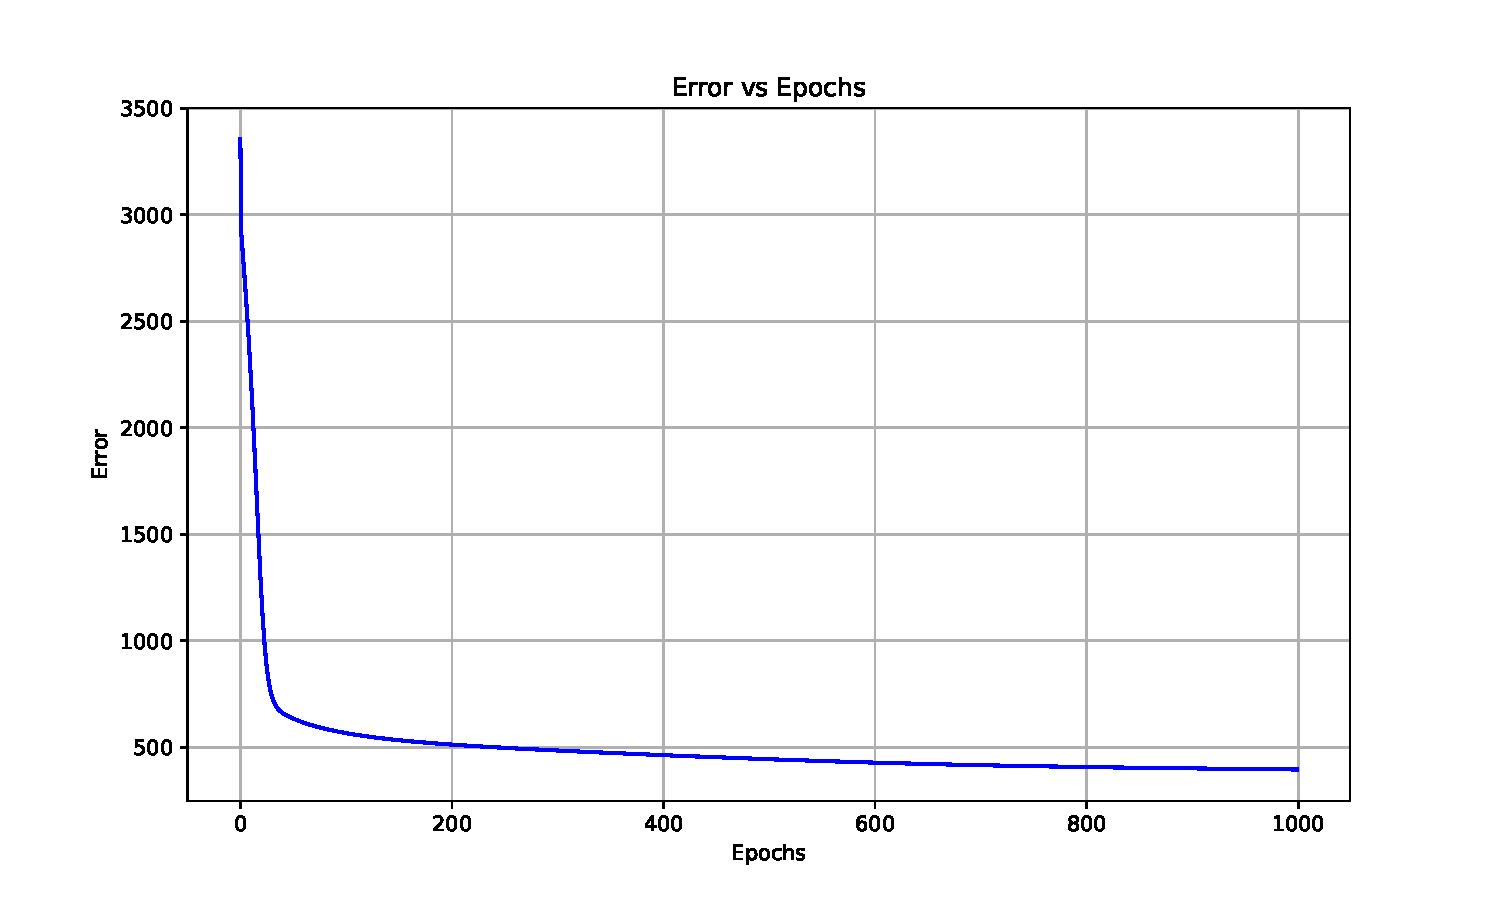
\includegraphics[width=0.8\textwidth, page=1]{pdfs/error_vs_epochs_0.1_1000.pdf}
    \caption{Error vs. Epochs}
    \label{fig:error_vs_epochs}
\end{figure}
This graph shows the average error of the network over the number of epochs.
The error was calculated with the mean squared error function.
The error decreases as the number of epochs increases, showing that the network is learning the patterns in the data.
The final MSE at epoch 1000 is about 410. This means the RMSE is about 20.25.
This interpretation is that the network is off by about 20.25 meters per second cubed on average off its true value.

\begin{figure}[H]
    \centering
    \includegraphics[width=0.8\textwidth, page=2]{pdfs/error_vs_epochs_0.1_1000.pdf}
    \caption{Predicted vs. Expected Output}
    \label{fig:error_vs_epochs2}
\end{figure}

\begin{figure}[H]
    \centering
    \includegraphics[width=0.8\textwidth, page=3]{pdfs/error_vs_epochs_0.1_1000.pdf}
    \caption{Correlation of Predicted vs. Expected Output}
    \label{fig:error_vs_epochs3}
\end{figure}

\begin{lstlisting}[language=Python]
back_prop_multi.py
    
    perceptronStructure = (7, [(16, 'sigmoid'),(16, 'sigmoid'), (1, 'sigmoid')])
    learningRate = 0.1
    epochs = 10000
    
\end{lstlisting}

\begin{figure}[H]
    \centering
    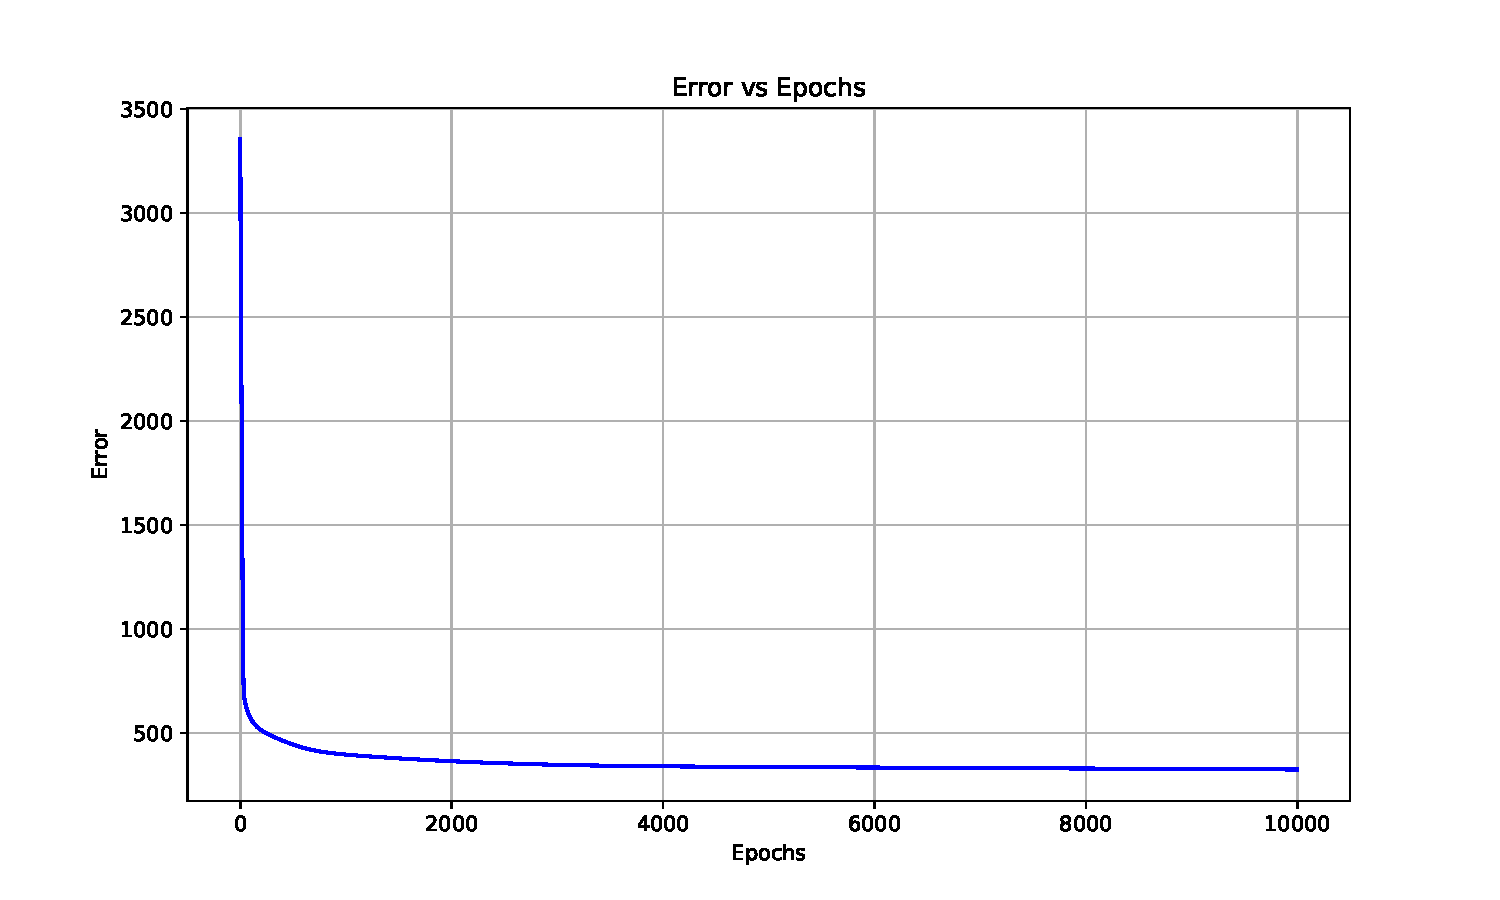
\includegraphics[width=0.8\textwidth, page=1]{pdfs/error_vs_epochs_0.1_10000.pdf}
    \caption{Error vs. Epochs}
    \label{fig:error_vs_epochs-2}
\end{figure}
The MSE in this graph is around 250, which means the RMSE is about 15.8.
This provides a much better result than the previous network, showing that the network is learning the patterns in the data.
However, we can see that the network stopped learning after about 5000 epochs, as the error does not decrease after this point.
We can alter the structure of the network and improve it to reduce the errors

\begin{figure}[H]
    \centering
    \includegraphics[width=0.8\textwidth, page=2]{pdfs/error_vs_epochs_0.1_10000.pdf}
    \caption{Predicted vs. Expected Output}
    \label{fig:error_vs_epochs2-2}
\end{figure}

Figure 2.6.5 clearly shows a better and more accurate prediction of the network compared to figure 2.6.2.

\begin{figure}[H]
    \centering
    \includegraphics[width=0.8\textwidth, page=3]{pdfs/error_vs_epochs_0.1_10000.pdf}
    \caption{Correlation of Predicted vs. Expected Output}
    \label{fig:error_vs_epochs3-2}
\end{figure}

The correlation of the network in figure 1.6.6 is much better than the correlation in figure 1.6.3.
The data is less skewed and the network is predicting the data more accurately.
\vspace{1em}
\newline
We can see that the network is learning the patterns in the data, but we can improve the network by changing the structure of the network.
To improve the data, we can code improvements to the network to make it more efficient and faster.
However, the code is slow to execute and the speed of the implementation needs to improved to make it more efficient.
There are also datapoints that are clearly outliers too, and these can be removed to improve the network.
Once these points are removed we may see a higher accuracy in the network.

\section{Object oriented implementation}

As previously mentioned, the data has many outliers that are affecting the network, and these need to be removed.
The previous parameters were:
\begin{lstlisting}[language=python]
data_cleaning.py

    iqrWeight = 1.5
    sdWeight = 2
    windowSize = 10
    replacementRange = 6

\end{lstlisting}
And these will be changed to:
\begin{lstlisting}[language=python]
data_cleaning.py
    
    iqrWeight = 1.4
    sdWeight = 1.6
    windowSize = 20
    replacementRange = 8
    
\end{lstlisting}
This removes 1559 data points from the dataset, which is 150\% more than the previous parameters.
\begin{figure}[H]
    \centering
    \includegraphics[width=0.8\textwidth, page=4]{pdfs/iqr1.4_sd1.6,ws20_rr8.pdf}
    \caption{Cleaned Skelton Data}
    \label{fig:Data_cleaned}
\end{figure}

We can then implement the network in an object-oriented way to make it more efficient and easier to use.

\begin{lstlisting}[language=Python]
back_prop_OO.py

    import numpy as np
    import pandas as pd

    class MLP:

        def __init__(self, dataSet:pd.DataFrame, nodeStructure:list[tuple], learningRate:float, trainingEpochs:int, PredictedColumn:str):
            '''Initialises the perceptron structure'''

            # Determine the number of input dimensions
            self.inputDimensions = (dataSet.shape[1]-2)

            # Normalise the training data
            self.dataFrameMin = dataSet[PredictedColumn].min()
            self.dataFrameMax = dataSet[PredictedColumn].max()
            self.dataSet = dataSet.copy()
            self.dataSet.iloc[:, 1:] = self.min_max_scaler(self.dataSet.iloc[:, 1:])

            # Split the data into training and testing
            self.trainingData = self.dataSet[dataSet['DATE'].dt.year.isin([1993, 1994])]
            self.testingData = self.dataSet[dataSet['DATE'].dt.year == 1995]


            # Store the structure of the network
            self.nodeStructure = nodeStructure
            self.learningRate = learningRate
            self.trainingEpochs = trainingEpochs

            # Create lists for weights and biases
            self.weightList = []
            self.biasList = []

            # Populate the structure lists
            previousLayer = self.inputDimensions

            for layer in self.nodeStructure:
                # Create matrices for the weights and biases
                weightMatrix = np.random.uniform(-1, 1, (previousLayer, layer[0]))
                biasMatrix = np.random.uniform(-1, 1, (1, layer[0]))

                # Append to the lists
                self.weightList.append(weightMatrix)
                self.biasList.append(biasMatrix)

                # Update the previous layer
                previousLayer = layer[0]

            # Create dataframe for storing the error per epoch
            self.epochErrorDF = pd.DataFrame(columns=['Epoch', 'Error'])

            # Create dataframe for storing the predictions
            self.predictionDF = pd.DataFrame(columns=['DATE', 'Skelton'])


        def train_network(self) -> pd.DataFrame:
        '''Function to train the neural network'''

        # Iterate through the training epochs
        for epoch in range(self.trainingEpochs):

            # Create a dataframe to store the mean error for the epoch
            meanErrorList = []

            # Convert data to numpy array
            inputDataArray = self.trainingData.iloc[:, 2:].values
            expectedOutputArray = self.trainingData.iloc[:, 1].values

            # Iterate though each day in the training data
            for i in range(len(inputDataArray)):

                # Split the data point into input and output
                inputData, expectedOutput = inputDataArray[i], expectedOutputArray[i]

                # Pass the data through the network
                activatedList, summedList = self.forward_pass(inputData) 

                meanErrorList.append(self.error_storing(expectedOutput, activatedList[-1]))

                # Backward pass through the network
                self.backward_pass(expectedOutput, summedList, activatedList, inputData)

            # Convert errors into dataframe
            meanErrorDF = pd.DataFrame({'Error' : meanErrorList})

            # Calculate the mean error for the epoch
            meanError = meanErrorDF['Error'].mean()

            # Store the mean error for the epoch
            newError = pd.DataFrame({'Epoch': [epoch], 'Error': [meanError]})
            self.epochErrorDF = pd.concat([self.epochErrorDF, newError], ignore_index=True)

            # Print the error for the epoch
            if epoch % 100 == 0:
                print(f'Epoch: {epoch}, Error: {meanError}')


\end{lstlisting}

The object oriented approach should hopefully increase speeds.
To be able to compare networks accurately, in terms of error and time taken, I will use the same machine and parameters to run the networks.
\begin{lstlisting}[language=Python]
back_prop_OO.py

    import time

    # Define the structure of the network
    nodeStructure = [(16, 'sigmoid'),(16, 'sigmoid'), (1, 'sigmoid')]

    # Define the learning rate and epochs
    learningRate = 0.1
    trainingEpochs = 10000

    # Fix random seed for reproducibility
    np.random.seed(42)

    start_time = time.time()

    if __name__ == '__main__':
        main()

    end_time = time.time()
    print(f'Time taken: {end_time - start_time} seconds')

\end{lstlisting}

These same parameters will be used for the object-oriented implementation and the previous implementation.

\begin{table}[h]
    \centering
    \begin{tabular}{|c|c|}
        \hline
        Objected Orientated & Prodcedural  \\
        \hline
        546 & 2154 \\
        \hline
    \end{tabular}
    \caption{Time taken to run 10,000 epochs in seconds}
    \label{tab:iqr_results}
\end{table}

The object-oriented implementation is much faster than the procedural implementation, with a speed increase of 75\%.
This is a significant improvement and shows that the object-oriented implementation is much more efficient.
\vspace{1em}
\newline
It is worth noting that the object-oriented implementation is not a perfect match in terms of each steps, as there were minor improvements made to the code to fix some issues.
However, the main structure of the code is the same, and the improvements made to the code are minor, and both return the same results.

\section{Batch Learning}
Batch learning is an improvement meant to speed up the learning process of the network.
Instead of updating the weights and biases after each data point, we can update the weights and biases after a batch of data points.
This relys on more efficient matrix calculations, rather than iteration.
\vspace{1em}
\newline
As well as offering an increase in speed computationaly, it can also offer an increase to the speed of learning (reduce the amount of epochs used).
This is because by averaging the error over a batch of data points, we can reduce the noise in the data and get a more accurate representation of the error.
This can help the network learn the patterns in the data more efficiently.

\begin{lstlisting}[language=Python]
back_prop_batch_learning.py

    class MLP:

        def __init__(self, dataSet:pd.DataFrame, nodeStructure:list[tuple], learningRate:float, trainingEpochs:int, PredictedColumn:str):
            '''Initialises the perceptron structure'''

            # Determine the number of input dimensions
            self.inputDimensions = (dataSet.shape[1]-2)

            # Normalise the training data
            self.dataFrameMin = dataSet[PredictedColumn].min()
            self.dataFrameMax = dataSet[PredictedColumn].max()
            self.dataSet = dataSet.copy()
            self.dataSet.iloc[:, 1:] = self.min_max_scaler(self.dataSet.iloc[:, 1:])

            # Reshape into a 3D array
            self.dataSet = self.dataSet.to_numpy().reshape(dataSet.shape[0], 1, dataSet.shape[1])

            # Split the data into training and testing
            self.trainingData = self.dataSet[dataSet['DATE'].dt.year.isin([1993, 1994])]
            self.testingData = self.dataSet[dataSet['DATE'].dt.year == 1995]


            # Store the structure of the network
            self.nodeStructure = nodeStructure
            self.learningRate = learningRate
            self.trainingEpochs = trainingEpochs

            # Create lists for weights and biases
            self.weightList = []
            self.biasList = []

            # Populate the structure lists
            previousLayer = self.inputDimensions

            for layer in self.nodeStructure:
                # Create matrices for the weights and biases
                weightMatrix = np.random.uniform(-1, 1, (previousLayer, layer[0]))
                biasMatrix = np.random.uniform(-1, 1, (1, layer[0]))

                # Append to the lists
                self.weightList.append(weightMatrix)
                self.biasList.append(biasMatrix)

                # Update the previous layer
                previousLayer = layer[0]

            # Create dataframe for storing the error per epoch
            self.epochErrorDF = pd.DataFrame(columns=['Epoch', 'Error'])

            # Create dataframe for storing the predictions
            self.predictionDF = pd.DataFrame(columns=['DATE', 'Skelton'])

        def train_network(self) -> pd.DataFrame:
            '''Function to train the neural network'''
    
            # Iterate through the training epochs
            for epoch in range(self.trainingEpochs):
    
                # Split the data point into input and output, maintaining the 3D structure
                inputData, expectedOutput = self.trainingData[:, :, 2:], self.trainingData[:, :, 1:2]
    
                # Pass the data through the network
                activatedList, summedList = self.forward_pass(inputData) 
    
                # Calculate the error of the network
                meanErrorList = self.error_storing(expectedOutput, activatedList[-1])
                
                # Reshape dimensions
                meanErrorList = meanErrorList.squeeze(axis=1)
    
                # Average the outputs
                meanErrorList = meanErrorList.mean(axis=1)
    
                # Backward pass through the network
                self.backward_pass(expectedOutput, summedList, activatedList, inputData)
    
                # Convert errors into dataframe
                meanErrorDF = pd.DataFrame({'Error' : meanErrorList})
    
                # Calculate the mean error for the epoch
                meanError = meanErrorDF['Error'].mean()
    
                # Store the mean error for the epoch
                newError = pd.DataFrame({'Epoch': [epoch], 'Error': [meanError]})
                self.epochErrorDF = pd.concat([self.epochErrorDF, newError], ignore_index=True)
    
                # Print the error for the epoch
                if epoch % 100 == 0:
                    print(f'Epoch: {epoch}, Error: {meanError}')

\end{lstlisting}

I chose to implement this by using pythons solution to mismatched dimensions, broadcasting.
This allows me to define all inputs and values at nodes ($S$, $\alpha$) as 3D arrays.
With broadcasting, I only need one weight matrix, saving space and computation time.
This is because the weight matrix can be broadcasted to the correct dimensions for each layer.
\vspace{1em}
\newline
When run with our testing structure:

\begin{table}[h]
    \centering
    \begin{tabular}{|c|c|}
        \hline
        Batch Learning & Objected Orientated  \\
        \hline
        70 & 546 \\
        \hline
    \end{tabular}
    \caption{Time taken to run 10,000 epochs in seconds}
    \label{tab:iqr_results}
\end{table}

This time was acheived when passing the whole dataset as a batch.
This is a significant improvement in speed, with a 87\% increase in speed.
This is a significant improvement and shows that the batch learning implementation is much more efficient.
However, the batch learning with the whole batch has a much higher error than the previous implementations.
\vspace{1em}
\newline
The batch learning implementation does not yield the same accuracy as prvious implementations due to the batch size.
Large batch sizes remove patterns that can be learnt from, and the network can not evolve or learn from these patterns as they are smoothed out.

\begin{figure}[H]
    \centering
    \includegraphics[width=0.8\textwidth, page=2]{pdfs/error_vs_epochs_0.1_10000.pdf}
    \caption{Predicted vs. Expected Output for non-Batrch Learning}
    \label{fig:error_vs_epochs2-3}
\end{figure}

\begin{figure}[H]
    \centering
    \includegraphics[width=0.8\textwidth, page=2]{pdfs/error_vs_epochs_0.1_10000_batch.pdf}
    \caption{Predicted vs. Expected Output for Batrch Learning}
    \label{fig:error_vs_epochs2-4}
\end{figure}

As clearly visible in figures 2.6.8 and 2.6.9, the batch learning implementation is not as accurate as the non-batch learning implementation.
We can however, alter the batch size, either statically or dynamically, therefor allowing for patters to be learnt from the data.
\begin{figure}[H]
    \centering
    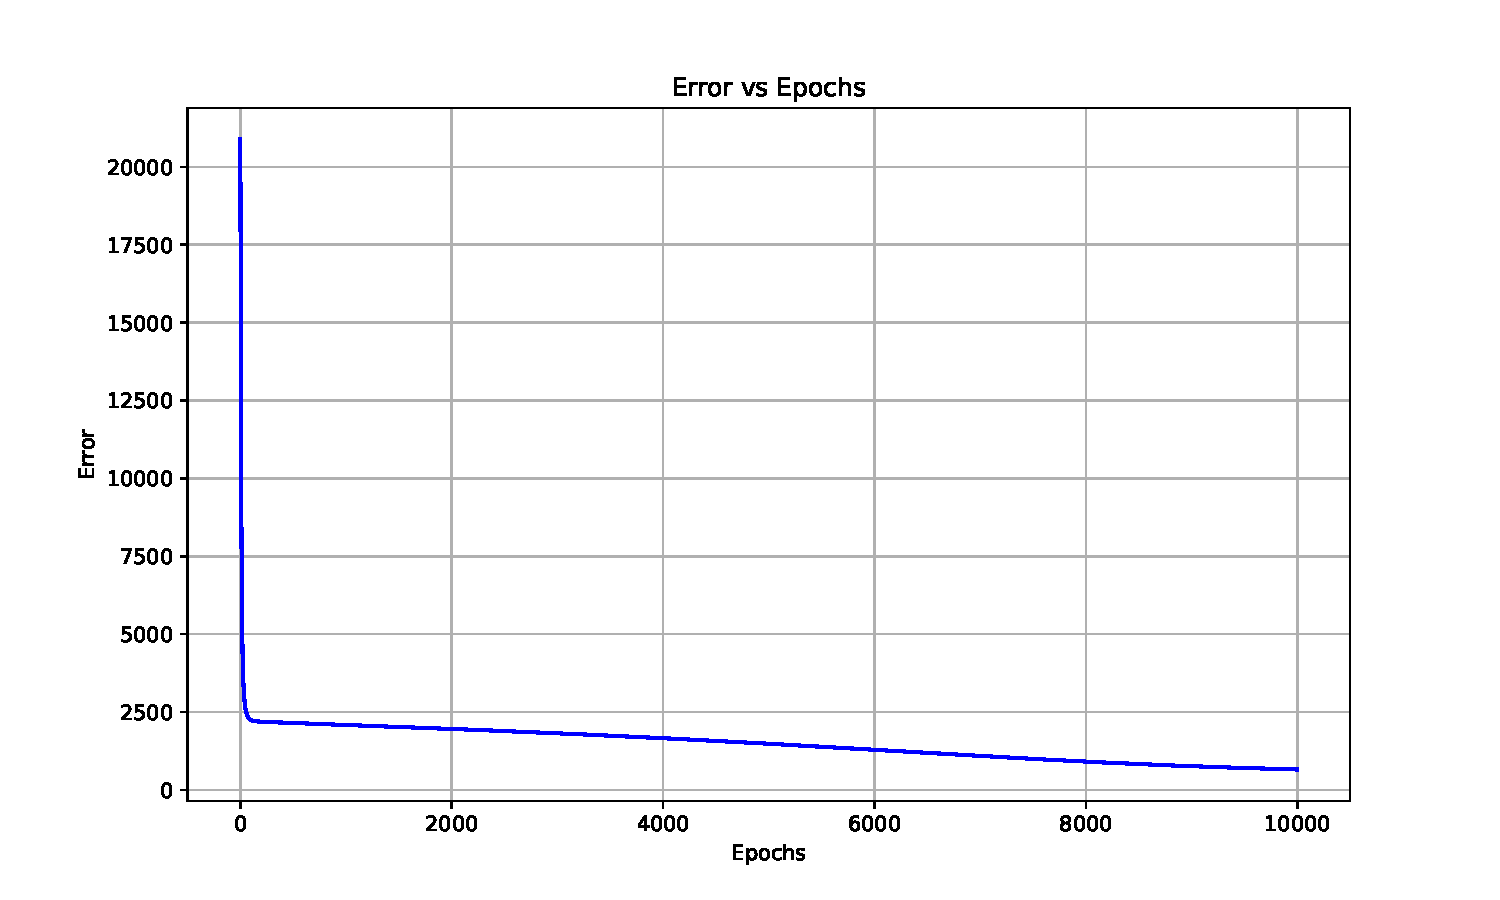
\includegraphics[width=0.8\textwidth, page=1]{pdfs/error_vs_epochs_0.1_10000_batch.pdf}
    \caption{Error vs. Epochs for Batch Learning}
    \label{fig:error_vs_epochsBatch}
\end{figure}

Using data from this graph, we can try to calculate the error of the gradient, so that when it stagnates, we can reduce the batch size.
This allows for fast learning before ending of accurate predictions.

\begin{lstlisting}[language=Python]
back_prop_batch_learning.py

    class MLP:

    def train_network(self) -> pd.DataFrame:
        '''Function to train the neural network'''

        # Iterate through the training epochs
        for epoch in range(self.trainingEpochs):

            # Define the batch data
            batchData = np.array_split(self.trainingData, self.batchSize)

            # Define the mean error list
            meanErrorList = []

            # Iterate through the batches
            for batch in batchData:

                # Split the data point into input and output, maintaining the 3D structure
                inputData, expectedOutput = batch[:, :, 2:], batch[:, :, 1:2]

                # Pass the data through the network
                activatedList, summedList = self.forward_pass(inputData) 

                # Calculate the error of the network
                meanErrorbatch = self.error_storing(expectedOutput, activatedList[-1])
                
                # Reshape dimensions
                meanErrorbatch = meanErrorbatch.squeeze(axis=1)

                # Average the outputs and store in the list
                meanErrorList.append(meanErrorbatch.mean())

                # Backward pass through the network
                self.backward_pass(expectedOutput, summedList, activatedList, inputData)


            # Convert errors into dataframe
            meanErrorDF = pd.DataFrame({'Error' : meanErrorList})

            # Calculate the mean error for the epoch
            meanError = meanErrorDF['Error'].mean()

            # Store the mean error for the epoch
            newError = pd.DataFrame({'Epoch': [epoch], 'Error': [meanError]})
            self.epochErrorDF = pd.concat([self.epochErrorDF, newError], ignore_index=True)

            # Only allow changes every 200 epochs to force the network to learn at certain points, and enforces at least 2 epochs
            if epoch % 200 == 0 and len(self.epochErrorDF) > 1:

                # Calculate the error gradient with respect to the batch size
                errorGradient = np.gradient(self.epochErrorDF['Error'])

                print(f'Error Gradient: {errorGradient[-1]}')

                # Doesn't allow batch size to be greater than the training data
                if self.batchSize == len(self.trainingData):
                    None

                # Increase the batch size
                elif abs(errorGradient[-1]) < 0.2:
                    self.batchSize = self.batchSize * 2

                    # Forces batch size to be the same as the training data
                    if self.batchSize > len(self.trainingData):
                        self.batchSize = len(self.trainingData)
    
\end{lstlisting}

This code allows for batch size to be dynamically decreased, so that when the error gradient stagnates, the batch size is reduced.
This allows for the network to learn more efficiently and accurately.

\begin{table}[H]
    \centering
    \begin{tabular}{|c|c|c|}
        \hline
        Batch Learning & Batch Learning with Dynamic Batch Size & Objected Orientated  \\
        \hline
        70 & 259 & 546\\
        \hline
    \end{tabular}
    \caption{Time taken to run 10,000 epochs in seconds}
    \label{tab:dynamicBatch}

\end{table}

\begin{table}[H]
    \centering
    \begin{tabular}{|c|c|c|}
        \hline
        Batch Learning & Batch Learning with Dynamic Batch Size & Objected Orientated  \\
        \hline
        665 & 295 & 250\\
        \hline
    \end{tabular}
    \caption{MSE at 10,000 epochs}
    \label{tab:dynamicBatch}

\end{table}

At the 10,000 epoch mark, the dynamic batch size does not reach the same error as the standard object-oriented implementation.
If trained for longer, it will reach the same point.
\begin{figure}[H]
    \centering
    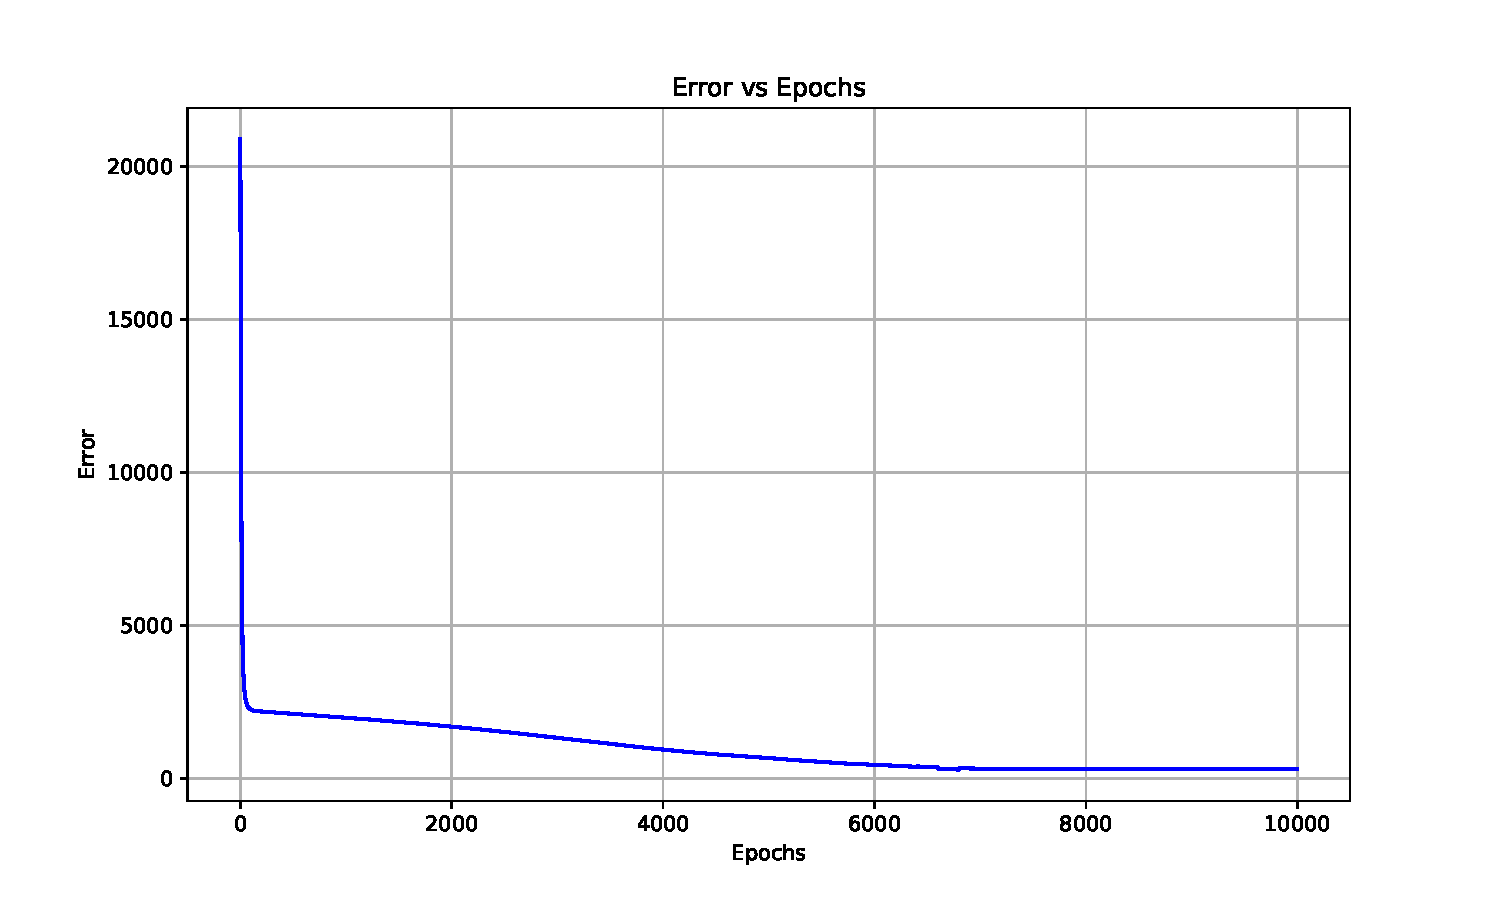
\includegraphics[width=0.8\textwidth, page=1]{pdfs/error_vs_epochs_0.1_10000_dynamic_batch.pdf}
    \caption{Error Gradient jumps in Dynamic Batch Size}
    \label{fig:error_vs_epochs2-3}
\end{figure}

However, the dynamic batch size implementation is much faster than the object-oriented implementation, with a 46\% increase in speed.
This is a significant improvement and shows that the dynamic batch size implementation is much more efficient.
As the batch size approches the size of the training data, the error will decrease, and the network will learn slower.
This means that for larger epochs, the speed increase is static, and not proportional to the amount of epochs.
As epochs inceases, the difference in speed between the dynamic batch size and the object-oriented implementation will decrease, and so will the error.
This implementation is best used for closing ground quickly and then fine-tuning the network with a smaller batch size.
\begin{figure}[H]
    \centering
    \includegraphics[width=0.8\textwidth, page=2]{pdfs/error_vs_epochs_0.1_10000_dynamic_batch.pdf}
    \caption{Predicted vs. Expected Output for Dynamic Batch Size} 
    \label{fig:error_vs_epochs2-3}
\end{figure}

With large numbers of epochs this implementation looses its speed advantage and becomes the same as thne object-oriented implementation.

\section{Momentum}
Momentum is a tequnique used to speed up the learning process of the network.
If the gradient of the error graph is heading in the same direction, the learning rate is increased, propelling the network to learn faster.
This compounds the changes to remove large errors and speed up the learning process.

\begin{equation}
    \text{Matrix }\omega^{k}_{nq}  :\omega'^{k}_{nq} = \omega^{k}_{nq} + \eta\cdot\alpha_{n}^{k-1}\cdot\delta^{k}_{q} + \Delta\omega^{k}_{nq}
\end{equation}
Where $\Delta\omega^{k}_{nq}$ is the momentum value.

\begin{lstlisting}[language=Python]
back_prop_momentum.py

    class MLP:

        def backward_pass(self, expectedOutput:np.array, summedList:np.array, activatedList:np.array, inputData:np.array):
            '''Function to pass data through the network'''

            # Calculate the delta values for the network
            deltaList = self.delta_calculator(expectedOutput, activatedList, summedList)


            #  Set previous output as input values
            previousOutput = inputData

            # Iterate through the layers of the network
            for layer in range(len(self.nodeStructure)):

                # Update the weights and biases for the layer
                weightUpdate  = ((np.transpose(previousOutput, (0, 2, 1)) @ deltaList[layer]) * self.learningRate)
                biasUpdate = (deltaList[layer] * self.learningRate)

                # Update the previous output
                previousOutput = activatedList[layer]

                # Momentum update
                momentumValue = (self.weightList[layer] - self.previousWeightList[layer]) * self.momentumConstant

                # Update the weights and biases
                self.weightList[layer] += (weightUpdate.mean(axis=0, dtype=np.float64) + momentumValue)
                self.biasList[layer] += biasUpdate.mean (axis=0, dtype=np.float64)

            # Momentum update
            self.previousWeightList = self.weightList

\end{lstlisting}
The code shows how the momentum value is implemented and included in the weight update.
As each weight update is a result of the last, this compounds the changes and speeds up the learning process.
However, at smaller changes, the momentum can cause the network to overshoot the minimum, and so the momentum constant must be carefully chosen.

\begin{figure}[H]
    \centering
    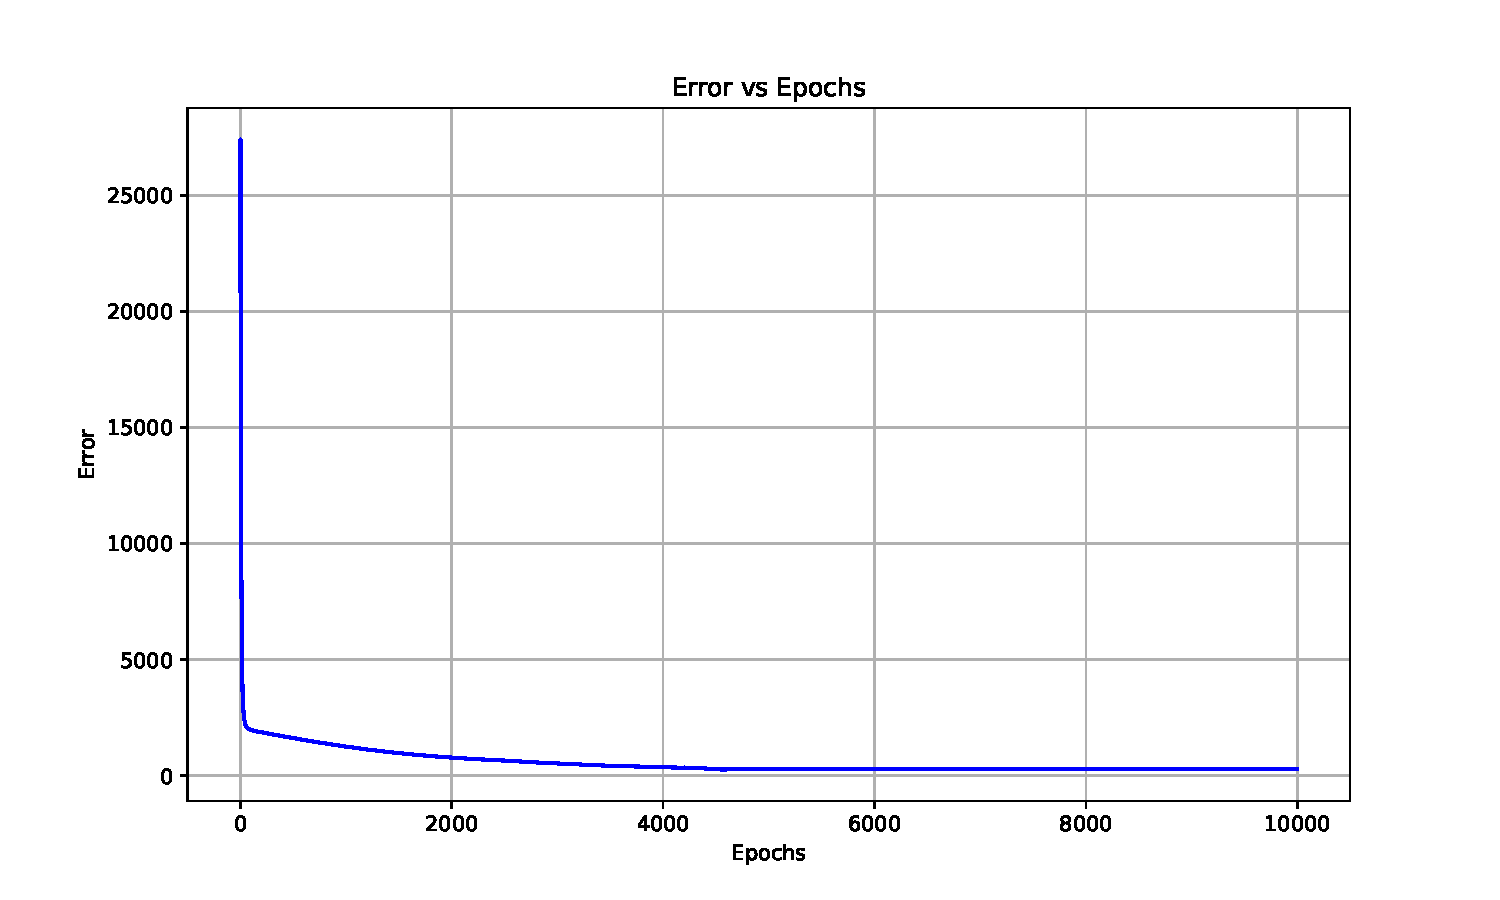
\includegraphics[width=0.8\textwidth, page=1]{pdfs/error_vs_epochs_0.1_10000_momentum.pdf}
    \caption{Error vs Epoch for Momentum} 
    \label{fig:error_vs_epochs2-3}
\end{figure}

\begin{table}[H]
    \centering
    \begin{tabular}{|c|c|}
        \hline
        Time Taken (seconds) & Error (MSE)  \\
        \hline
        407 & 287 \\
        \hline
    \end{tabular}
    \caption{statistics for 10,000 epochs of Momentum}
    \label{tab:dynamicBatch}

\end{table}

\begin{figure}[H]
    \centering
    \includegraphics[width=0.8\textwidth, page=2]{pdfs/error_vs_epochs_0.1_10000_momentum.pdf}
    \caption{Predicted vs Expected for Momentum} 
    \label{fig:error_vs_epochs2-3}
\end{figure}

This implementation tells us that Momentum allows us to reach lower errors faster, but then struggles to adapt after that point.
To help adjust this, we can reduce the momentum constant afteer we reach a certain gradient, just as with the batch learning implementation.
This can help us to fine-tune the network and reach a lower error.
While assessing this, I noticed my implementation of the gradient for lower batches was incorrect, as it use the whole gradient, not the local gradient.
This rapidly increases batch size, which is not efficient or effective.

\begin{lstlisting}[language=Python]
back_prop_momentum.py

    class mlp

        def train_network(self) -> pd.DataFrame:
            '''Function to train the neural network'''

            # Iterate through the training epochs
            for epoch in range(self.trainingEpochs):

                # Define the batch data
                batchData = np.array_split(self.trainingData, self.batchSize)

                # Define the mean error list
                meanErrorList = []

                # Iterate through the batches
                for batch in batchData:

                    # Split the data point into input and output, maintaining the 3D structure
                    inputData, expectedOutput = batch[:, :, 2:], batch[:, :, 1:2]

                    # Pass the data through the network
                    activatedList, summedList = self.forward_pass(inputData) 

                    # Calculate the error of the network
                    meanErrorbatch = self.error_storing(expectedOutput, activatedList[-1])
                    
                    # Reshape dimensions
                    meanErrorbatch = meanErrorbatch.squeeze(axis=1)

                    # Average the outputs and store in the list
                    meanErrorList.append(meanErrorbatch.mean())

                    # Backward pass through the network
                    self.backward_pass(expectedOutput, summedList, activatedList, inputData)


                # Convert errors into dataframe
                meanErrorDF = pd.DataFrame({'Error' : meanErrorList})

                # Calculate the mean error for the epoch
                meanError = meanErrorDF['Error'].mean()

                # Store the mean error for the epoch
                newError = pd.DataFrame({'Epoch': [epoch], 'Error': [meanError]})
                self.epochErrorDF = pd.concat([self.epochErrorDF, newError], ignore_index=True)


                # Only allow changes every 200 epochs to force the network to learn at certain points, and enforces at least 2 epochs
                if epoch % 200 == 0 and len(self.epochErrorDF) > 1:

                    # Define the last 200 points for an accurate gradient
                    recentErrors = self.epochErrorDF['Error'][-200:] if len(self.epochErrorDF) >= 200 else self.epochErrorDF['Error']

                    # Calculate the error gradient with respect to the batch size
                    errorGradient = np.gradient(recentErrors)

                    print(f'Error Gradient: {errorGradient[-1]}')

                    # Doesn't allow batch size to be greater than the training data
                    if self.batchSize == len(self.trainingData):
                        None

                    # Increase the batch size
                    elif abs(errorGradient[-1]) < 0.2:
                        self.batchSize = self.batchSize * 2
                        self.momentumConstant = self.momentumConstant * 0.6

                        # Forces batch size to be the same as the training data
                        if self.batchSize > len(self.trainingData):
                            self.batchSize = len(self.trainingData)


                # Print the error for the epoch
                if epoch % 100 == 0:
                    print(f'Epoch: {epoch}, Error: {meanError}, Batch Size: {self.batchSize}')
    
\end{lstlisting}

This is my dynamic reduction in momentum constant, which allows for the network to learn faster and then fine-tune the network.

\begin{table}[H]
    \centering
    \begin{tabular}{|c|c|}
        \hline
        Time Taken (seconds) & Error (MSE)  \\
        \hline
        400 & 287 \\
        \hline
    \end{tabular}
    \caption{statistics for 10,000 epochs of Dynamic Momentum}
    \label{tab:dynamicMomentum}

\end{table}

This improvement is not very significant, as the only increase is it is 7 seconds faster, which is a 1.7\% increase in speed.
In the last 5000 epochs, the MSE changed by 5. There was also a low point just before at 276, which was skipped over.
The take-away from this is that the smaller the error, the slower it learns.

\begin{figure}[H]
    \centering
    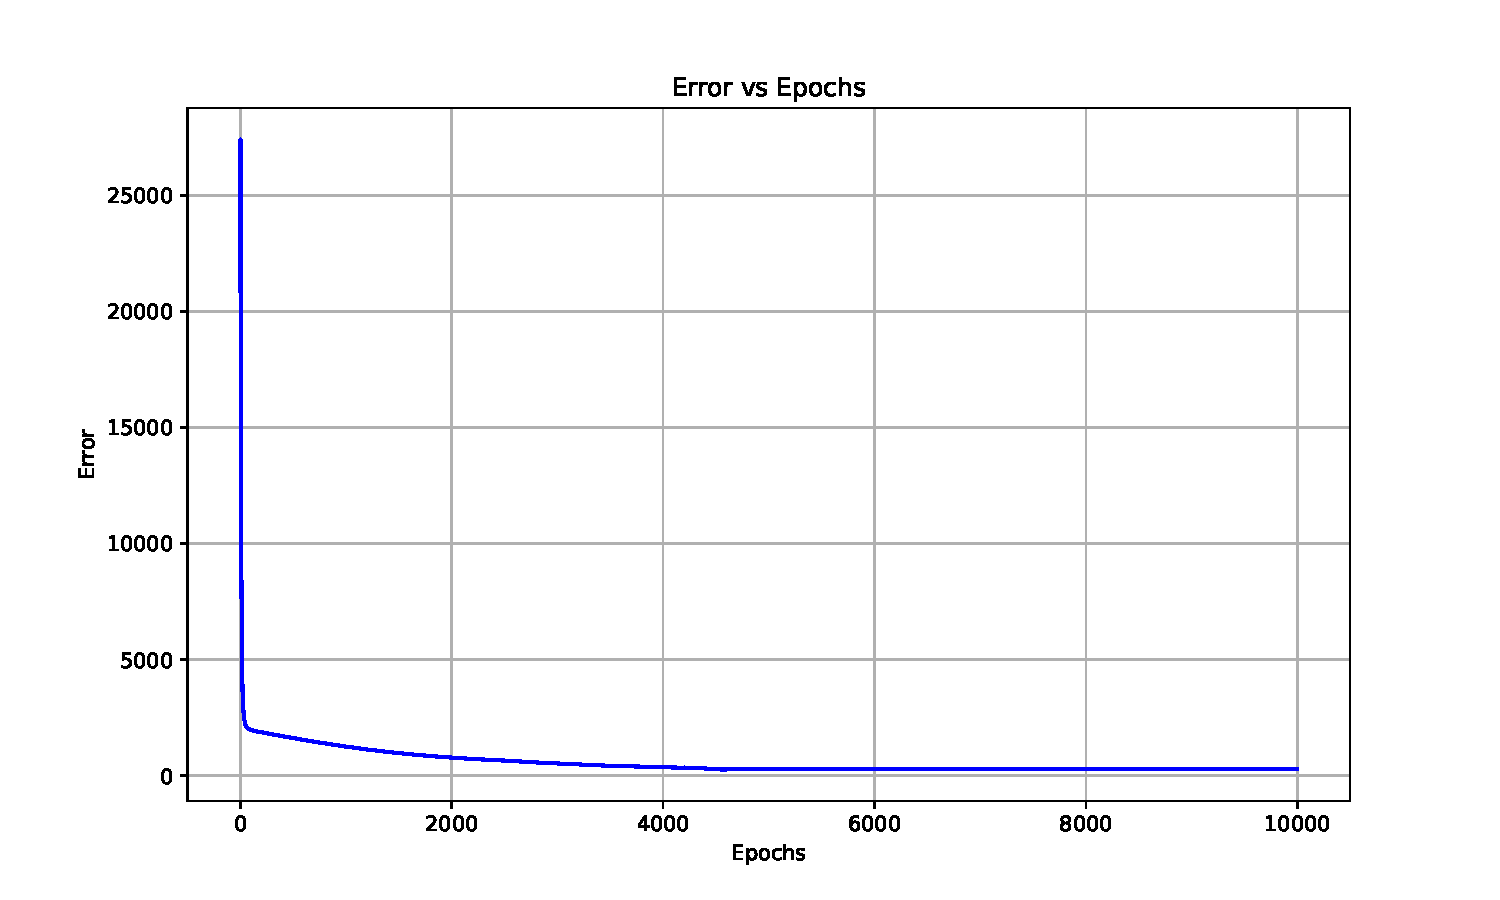
\includegraphics[width=0.8\textwidth, page=1]{pdfs/error_vs_epochs_0.1_1000_dynamic_momentum.pdf}
    \caption{Error vs Epoch for Dynamic Momentum} 
    \label{fig:error_vs_epochsD-2}
\end{figure}

\section{Bold Driver}

Bold driver is a tequnique that allows us to increase the learning rate when the gradient flattens out, allowing our network to still learn efficiently.
This can be done with bounds and dynamic learning rate, which can be adjusted to the gradient of the error.
\vspace{1em}
\newline
Bold drivers counter part is Anealing. 
This is where the learning rate is decreased as the gradient flatterns to help even out the network and stabalise it.
This helps you reach a minimum point quicker and then not overshoot it, but it can also slow down the learning process.
As my networks are already stable and are suffering from insifficient learning, I will not be implementing Anealing.

\begin{lstlisting}[language=Python]
back_prop_bold_driver.py

    class MLP:

        def __init__(self, dataSet:pd.DataFrame, nodeStructure:list[tuple], learningRate:float, trainingEpochs:int, PredictedColumn:str):
            '''Initialises the perceptron structure'''

            # Create Bold Driver Learning Rate
            self.boldDriverLearningRate = learningRate
            self.boldDriverCap = 0.8
            self.boldDriverIncrease = 1.2

        def train_network(self) -> pd.DataFrame:
            '''Function to train the neural network''' 

            # Only allow changes every 200 epochs to force the network to learn at certain points, and enforces at least 2 epochs
            if epoch % 200 == 0 and len(self.epochErrorDF) > 1:

                # Define the last 200 points for an accurate gradient
                recentErrors = self.epochErrorDF['Error'][-200:] if len(self.epochErrorDF) >= 200 else self.epochErrorDF['Error']

                # Calculate the error gradient with respect to the batch size
                errorGradient = np.gradient(recentErrors)

                print(f'Error Gradient: {errorGradient[-1]}')

                # Doesn't allow batch size to be greater than the training data
                if self.batchSize == len(self.trainingData):
                    None

                # Increase the batch size
                elif abs(errorGradient[-1]) < 0.3:
                    self.batchSize = self.batchSize * 2
                    self.momentumConstant = self.momentumConstant * 0.6

                    # Forces batch size to be the same as the training data
                    if self.batchSize > len(self.trainingData):
                        self.batchSize = len(self.trainingData)

                # Update the learning rate
                if abs(errorGradient[-1]) < 0.07:
                    self.boldDriverLearningRate = self.boldDriverLearningRate * self.boldDriverIncrease

                    # Caps the learning rate 
                    if self.boldDriverLearningRate > (1+self.boldDriverCap)*self.learningRate:
                        self.boldDriverLearningRate = (1+self.boldDriverCap)*self.learningRat

\end{lstlisting}

This code shows how the bold driver learning rate is implemented and included in the weight update.

\begin{table}[H]
    \centering
    \begin{tabular}{|c|c|}
        \hline
        Time Taken (seconds) & Error (MSE)  \\
        \hline
        434 & 282 \\
        \hline
    \end{tabular}
    \caption{statistics for 10,000 epochs of Bold Driver}
    \label{tab:dynamicMomentum}

\end{table}

\begin{figure}[H]
    \centering
    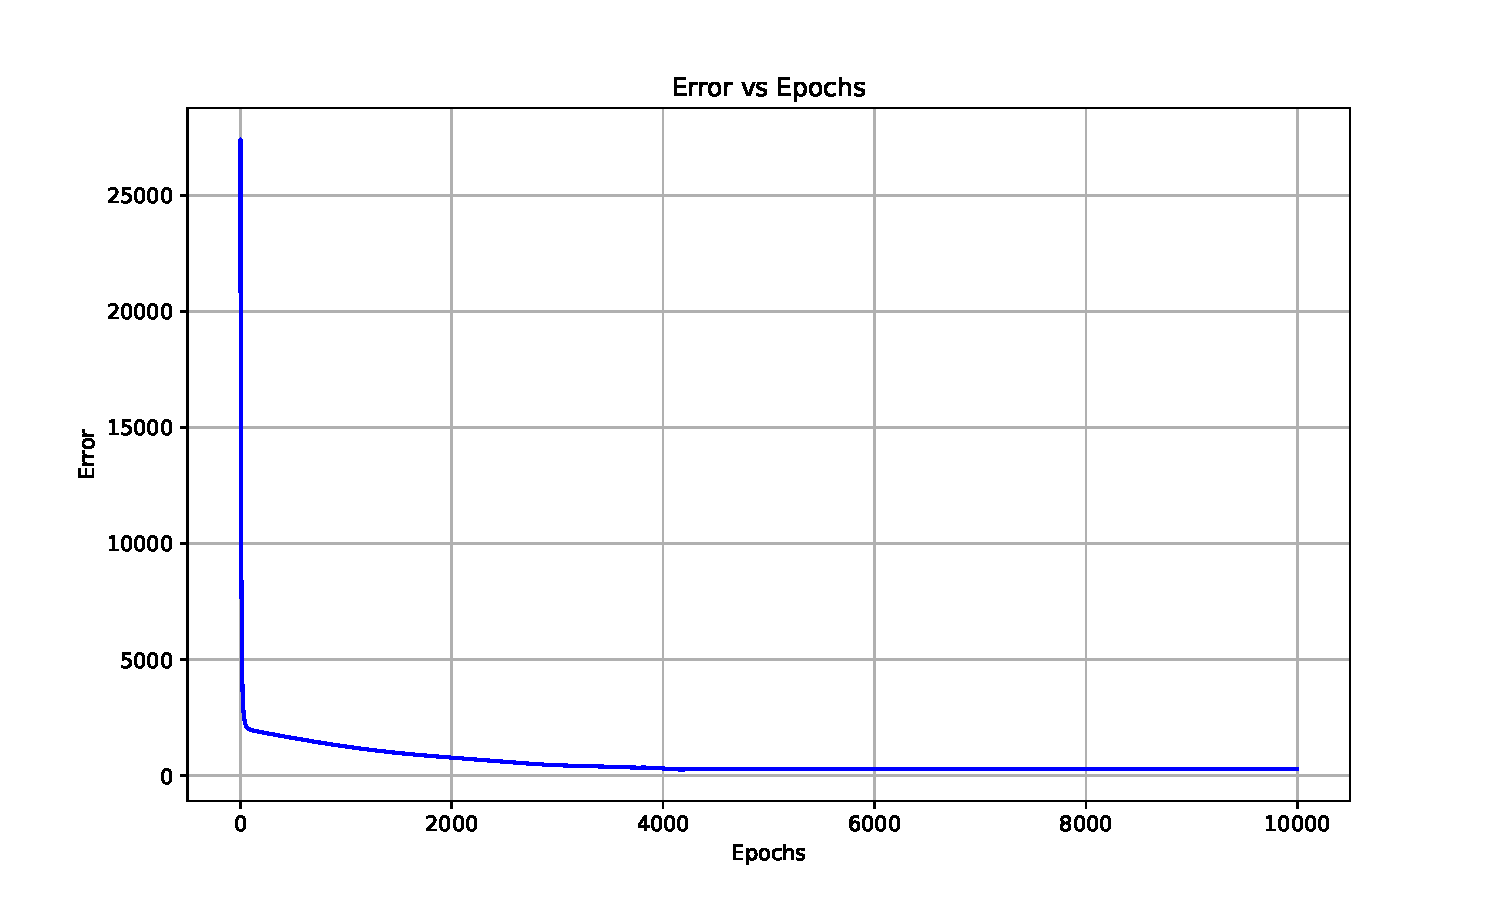
\includegraphics[width=0.8\textwidth, page=1]{pdfs/error_vs_epochs_0.1_10000_bold_driver.pdf}
    \caption{Error vs Epoch for Bold Driver} 
    \label{fig:error_vs_epochsD-2}
\end{figure}

The bold driver implementation does reduce the error, but not significantly.
It is possible our bold driver constants are not extreme enough, and so the learning rate is not changing enough.

\begin{lstlisting}[language=Python]
back_prop_bold_driver.py

    self.boldDriverCap = 20 
    
\end{lstlisting}
By increasing the cap, we can allow the network to learn more at these lower gradients.

\begin{table}[H]
    \centering
    \begin{tabular}{|c|c|}
        \hline
        Time Taken (seconds) & Error (MSE)  \\
        \hline
        371 & 238 \\
        \hline
    \end{tabular}
    \caption{statistics for 10,000 epochs of Bold Driver}
    \label{tab:dynamicMomentum2}

\end{table}

This is the best result so far, with a 14\% increase in speed and a 16\% decrease in error.
This is a significant improvement and shows that the bold driver implementation is much more efficient.

\begin{figure}[H]
    \centering
    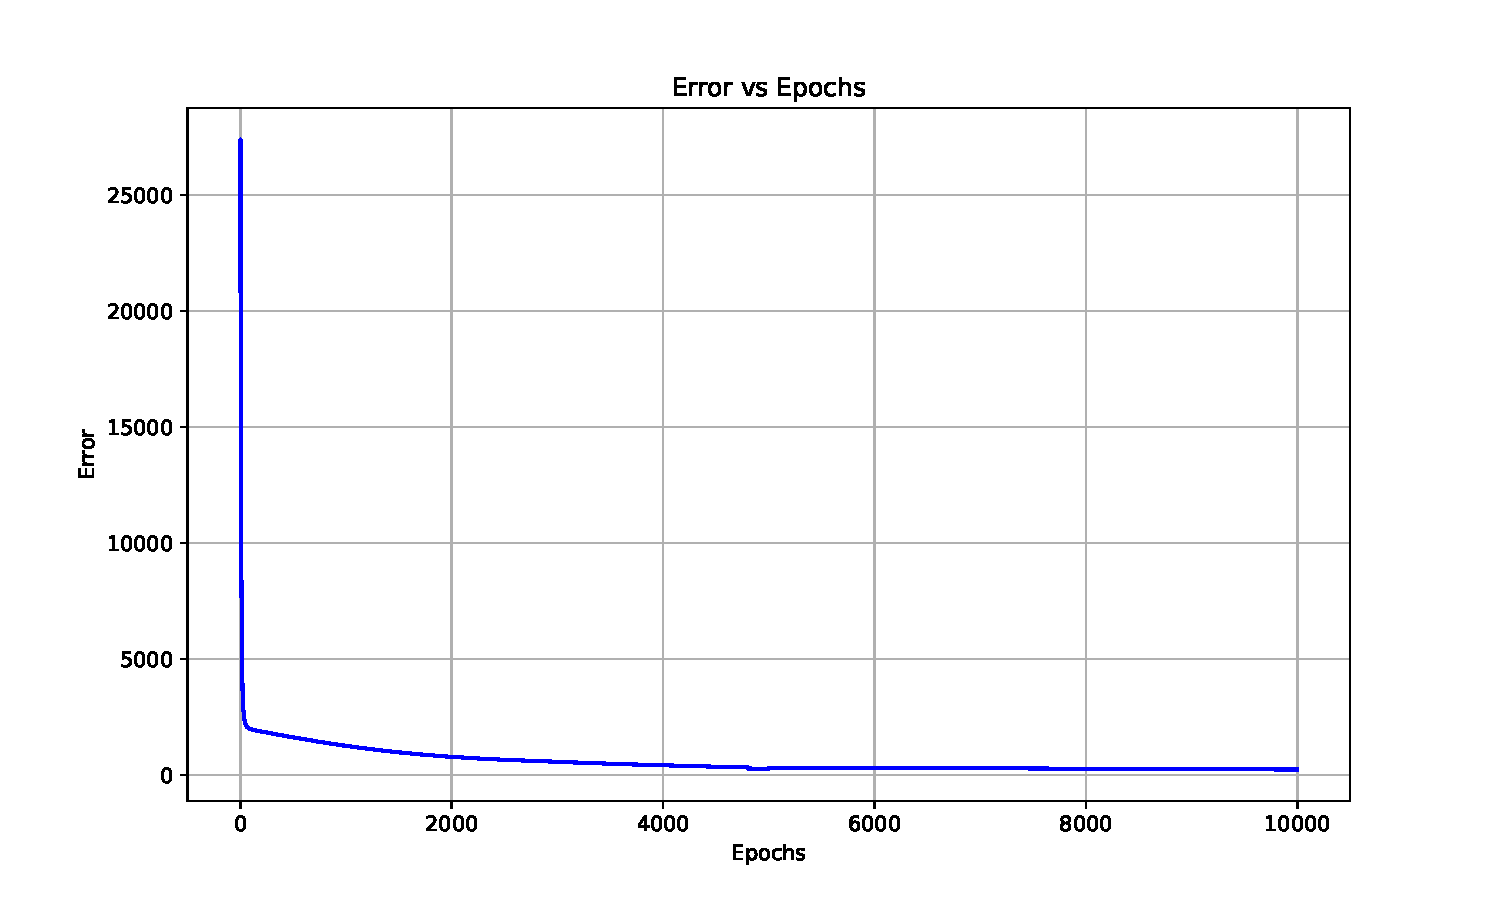
\includegraphics[width=0.8\textwidth, page=1]{pdfs/error_vs_epochs_0.1_10000_bold_driver_2.pdf}
    \caption{Error vs Epoch for Bold Driver (2$^{nd}$ Implementation)}  
    \label{fig:error_vs_epochsD-2}
\end{figure}

\begin{figure}[H]
    \centering
    \includegraphics[width=0.8\textwidth, page=2]{pdfs/error_vs_epochs_0.1_10000_bold_driver_2.pdf}
    \caption{Predicted vs Expected for Bold Driver (2$^{nd}$ Implementation)} 
    \label{fig:error_vs_epochsD-2}
\end{figure}

\section{Weight Decay}

Weight decay incetiveses the network to produce smaller weights, which can help to prevent overfitting.
It does this by adding a penalty term to error function, which is proportional to the size of the weights.

\begin{equation}
    \text{Matrix }\omega^{k}_{nq}  :\omega'^{k}_{nq} = \omega^{k}_{nq} + \eta\cdot\alpha_{n}^{k-1}\cdot\delta^{k}_{q} + \Delta\omega^{k}_{nq} - \rho \omega^{k}_{nq}
\end{equation}
Where $\rho \omega^{k}_{nq}$ is the weight decay term.
\vspace{1em}
\newline
This term forces weights to be much smaller, and so the network is less likely to overfit.

\begin{lstlisting}[language=Python]
back_prop_weight_decay.py

    class MLP:
        def __init__(self, dataSet:pd.DataFrame, nodeStructure:list[tuple], learningRate:float, trainingEpochs:int, PredictedColumn:str):
            '''Initialises the perceptron structure'''

            # Create weight decay constant
            self.weightDecay = 0.0001

        def backward_pass(self, expectedOutput:np.array, summedList:np.array, activatedList:np.array, inputData:np.array):
            '''Function to pass data through the network'''
    
            # Calculate the delta values for the network
            deltaList = self.delta_calculator(expectedOutput, activatedList, summedList)
    
    
            #  Set previous output as input values
            previousOutput = inputData
    
            # Iterate through the layers of the network
            for layer in range(len(self.nodeStructure)):
    
                # Update the weights and biases for the layer
                weightUpdate  = ((np.transpose(previousOutput, (0, 2, 1)) @ deltaList[layer]) * self.boldDriverLearningRate)
                biasUpdate = (deltaList[layer] * self.boldDriverLearningRate)
    
                # Update the previous output
                previousOutput = activatedList[layer]
    
                # Momentum update
                momentumValue = (self.weightList[layer] - self.previousWeightList[layer]) * self.momentumConstant
    
                # Weight Decay update
                weightDecay = self.weightList[layer] * self.weightDecay
    
                # Update the weights and biases
                self.weightList[layer] += (weightUpdate.mean(axis=0, dtype=np.float64) + momentumValue - weightDecay)
                self.biasList[layer] += biasUpdate.mean (axis=0, dtype=np.float64)
    
            # Momentum update
            self.previousWeightList = self.weightList
    
\end{lstlisting}

This code shows how the weight decay term is implemented and included in the weight update.

\begin{table}[H]
    \centering
    \begin{tabular}{|c|c|}
        \hline
        Time Taken (seconds) & Error (MSE)  \\
        \hline
        405 & 1313 \\
        \hline
    \end{tabular}
    \caption{statistics for 10,000 epochs of Weight Decay}
    \label{tab:dynamicMomentum}

\end{table}

This is the worst result so far, with a 361\% increase in error. 
This may be due to the weight decay term being too large, and so the network is not learning effectively.

\begin{figure}[H]
    \centering
    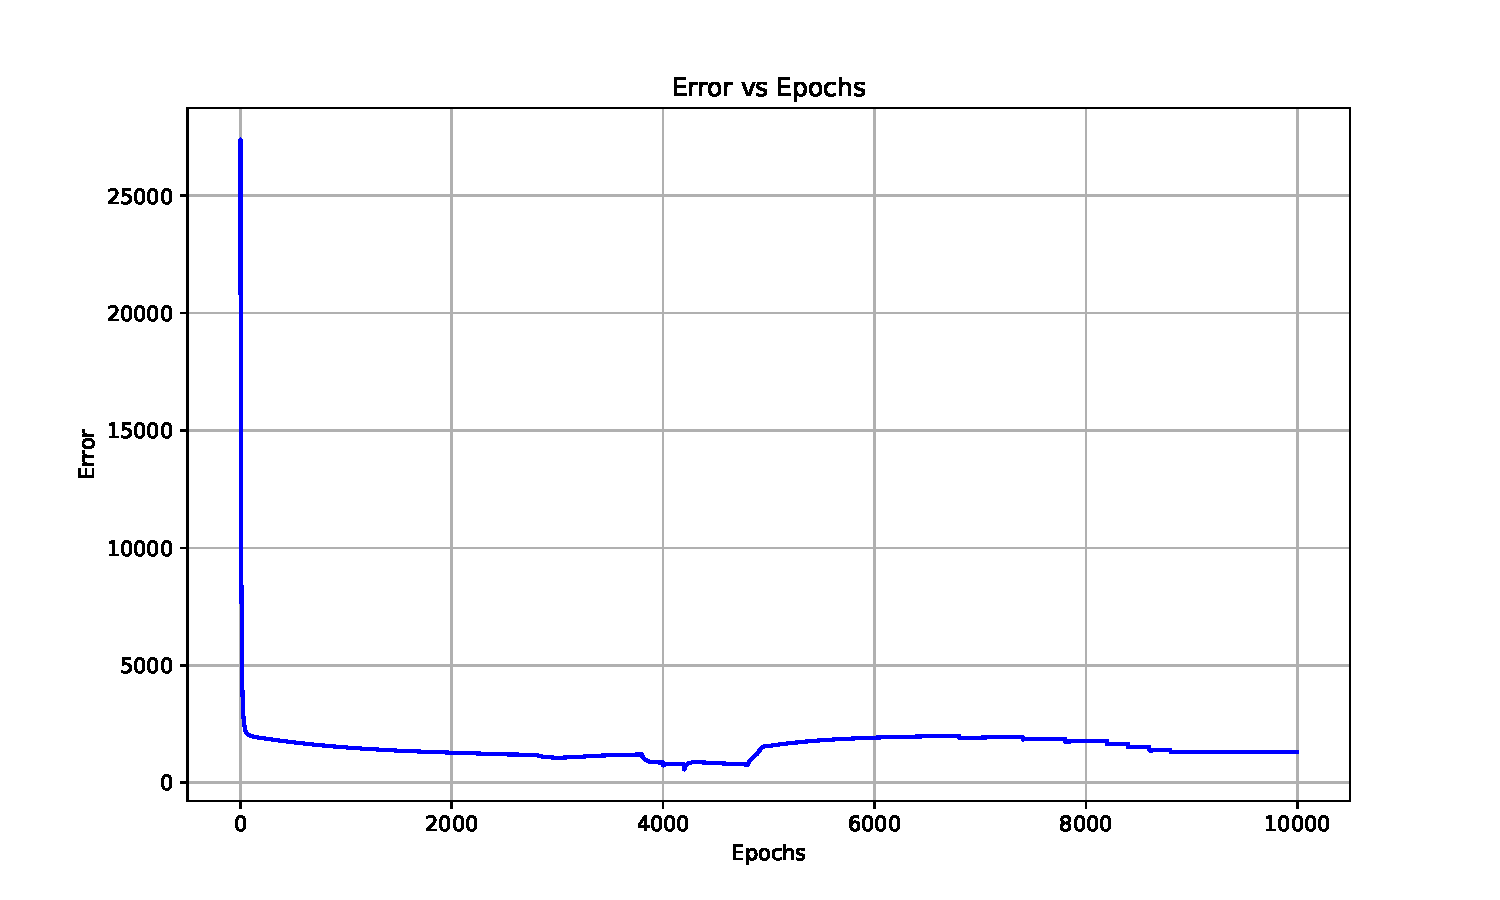
\includegraphics[width=0.8\textwidth, page=1]{pdfs/error_vs_epochs_0.1_10000_weightDecay1.pdf}
    \caption{Error vs Epoch for Weight Decay} 
    \label{fig:error_vs_epochsD-2}
\end{figure}

\begin{lstlisting}[language=Python]
back_prop_weight_decay.py

    self.weightDecay = 0.00001
\end{lstlisting}

By reducing the weight decay term, we can allow the network to learn more effectively.

\begin{table}[H]
    \centering
    \begin{tabular}{|c|c|}
        \hline
        Time Taken (seconds) & Error (MSE)  \\
        \hline
        375 & 303 \\
        \hline
    \end{tabular}
    \caption{statistics for 10,000 epochs of Weight Decay (2$^{nd}$ Implementation)}
    \label{tab:dynamicMomentum}

\end{table}

These results do not match the results without the weight decay as they only got worse.
I do not beleive that the network suffered from overfitting in previous implementations, and so the weight decay term was not needed.
For this reason, I will not be using weight decay in my final implementation.

\begin{figure}[H]
    \centering
    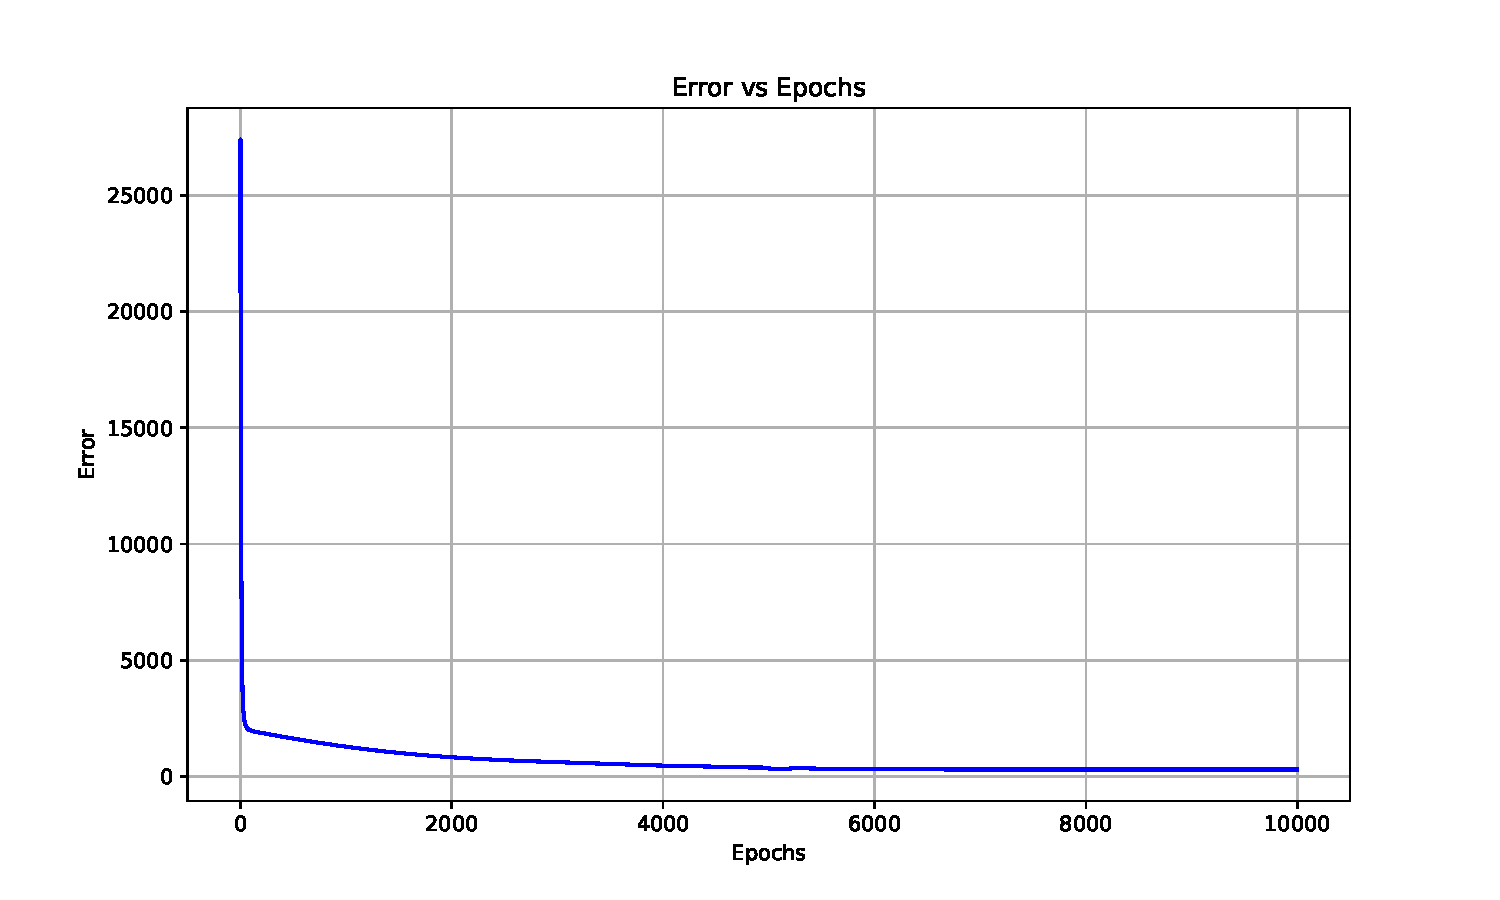
\includegraphics[width=0.8\textwidth, page=1]{pdfs/error_vs_epochs_0.1_10000_weightDecay2.pdf}
    \caption{Error vs Epoch for Weight Decay (2$^{nd}$ Implementation)} 
    \label{fig:error_vs_epochsD-2}
\end{figure}

\begin{figure}[H]
    \centering
    \includegraphics[width=0.8\textwidth, page=2]{pdfs/error_vs_epochs_0.1_10000_weightDecay2.pdf}
    \caption{Predicted vs Expected for Weight Decay (2$^{nd}$ Implementation)} 
    \label{fig:error_vs_epochsD-2}
\end{figure}

\section{Line Searching}

Learn searching is about using the gradient to adjust the learning rate of network to be more efficient and avoid overshooting the minimum.
We can define our output as a function of the learning rate and direction of the gradient.
\begin{equation}
O_k = O_{k-1} + \sigma d_k
\end{equation}
Where $O_k$ is the output, $O_{k-1}$ is the previous output, $\sigma$ is the learning rate and $d_k$ is the direction of the gradient.
\space{1em}
\newline
As we are optimising in terms of the learning rate, we can frame this as a minimisation problem of function $\phi$
\begin{equation}
\phi(\sigma) = f(O_{k-1} + \sigma d_k)
\end{equation}
Where $\phi$ is the function we are trying to minimise, $f$ is the function we are trying to optimise.
This means that we can use the gradient of $\phi$ to find the optimal learning rate as we use it to find the minimum of the function.
\begin{lstlisting}[language=Python]
back_prop_line_search.py

    class MLP:

        def line_search(self, expectedOutput:np.array, activatedList:np.array, summedList:np.array, inputData:np.array):
            '''Function to perform a line search and optimise the learning rate'''

            # Define the next two steps
            learningRateAlpha = self.learningRate
            learningRateBeta = self.learningRate * 50

            # Define the initial error and delta list
            deltaList, structureCost = self.delta_calculator(expectedOutput, activatedList, summedList)

            # Calculate the weights for the first step

            # Calculate the forward pass for the first step
            activatedListAlpha, summedListAlpha = self.forward_pass(inputData, self.weightList, self.biasList)

            # Calculate the error for the first step
            structureCostAlpha = self.error_storing(expectedOutput, activatedListAlpha[-1])

            # Calculate the weights for the second step

            # Calculate the forward pass for the second step
            activatedListBeta, summedListBeta = self.forward_pass(inputData, self.weightList, self.biasList)

            # Calculate the error for the second step
            structureCostBeta = self.error_storing(expectedOutput, activatedListBeta[-1])

            # Use a quadratic model to approximate the minimum learning rate
            X = np.array([
                [0**2, 0, 1],
                [learningRateAlpha**2, learningRateAlpha, 1],
                [learningRateBeta**2, learningRateBeta, 1]
            ])
            
            
            Y = np.array([structureCost.mean(), structureCostAlpha.mean(), structureCostBeta.mean()])
            
            # Solve for quadratic coefficients [a, b, c]
            a, b, c = np.linalg.solve(X, Y)
            
            # Compute the minimum learning rate
            stepSize = -b / (2 * a)

            # Calculate the backwards pass for the chose step size
            newWeightList, newBiasList = self.backward_pass(activatedList, inputData, stepSize, deltaList)

            self.weightList = newWeightList
            self.biasList = newBiasList

            # Momentum update
            self.previousWeightList = newWeightList

            def backward_pass(self, activatedList:np.array, inputData:np.array, lineSearchConstant:float, deltaList:np.array):
                '''Function to pass data through the network'''
        
                # Create a list for the temporary weights and biases
                temporaryWeightList = []
                temporaryBiasList = []
        
                #  Set previous output as input values
                previousOutput = inputData
        
                # Define the step size for the line search
                stepSize = self.boldDriverLearningRate * lineSearchConstant
        
                # Iterate through the layers of the network
                for layer in range(len(self.nodeStructure)):
        
                    # Update the weights and biases for the layer
                    weightUpdate  = ((np.transpose(previousOutput, (0, 2, 1)) @ deltaList[layer]) * stepSize)
                    biasUpdate = (deltaList[layer] * stepSize)
        
                    # Update the previous output
                    previousOutput = activatedList[layer]
        
                    # Momentum update
                    momentumValue = (self.weightList[layer] - self.previousWeightList[layer]) * self.momentumConstant
        
                    # Update the weights and biases
                    temporaryWeightList.append(self.weightList[layer] + (weightUpdate.mean(axis=0, dtype=np.float64) + momentumValue))
                    temporaryBiasList.append(self.biasList[layer] + biasUpdate.mean (axis=0, dtype=np.float64))
        
                return temporaryWeightList, temporaryBiasList
        
\end{lstlisting}
My implementation of $\phi$ is to use the current cost, along with 2 potential costs to approximate the minimum of a quadratic function.
This minumum will be used as the step size for the line search and then used to update our weights.
This is a costly operation, as it requires 3 backward passes and 3 forward passes per input.
With the batch learning, I hope to mitigate the cost of this operation.

\begin{table}[H]
    \centering
    \begin{tabular}{|c|c|}
        \hline
        Time Taken (seconds) & Error (MSE)  \\
        \hline
        805 & 170 \\
        \hline
    \end{tabular}
    \caption{statistics for 10,000 epochs of Line Searching}
    \label{tab:dynamicMomentum}

\end{table}

This is the best result so far, but with an expected increase in time taken.

\begin{figure}[H]
    \centering
    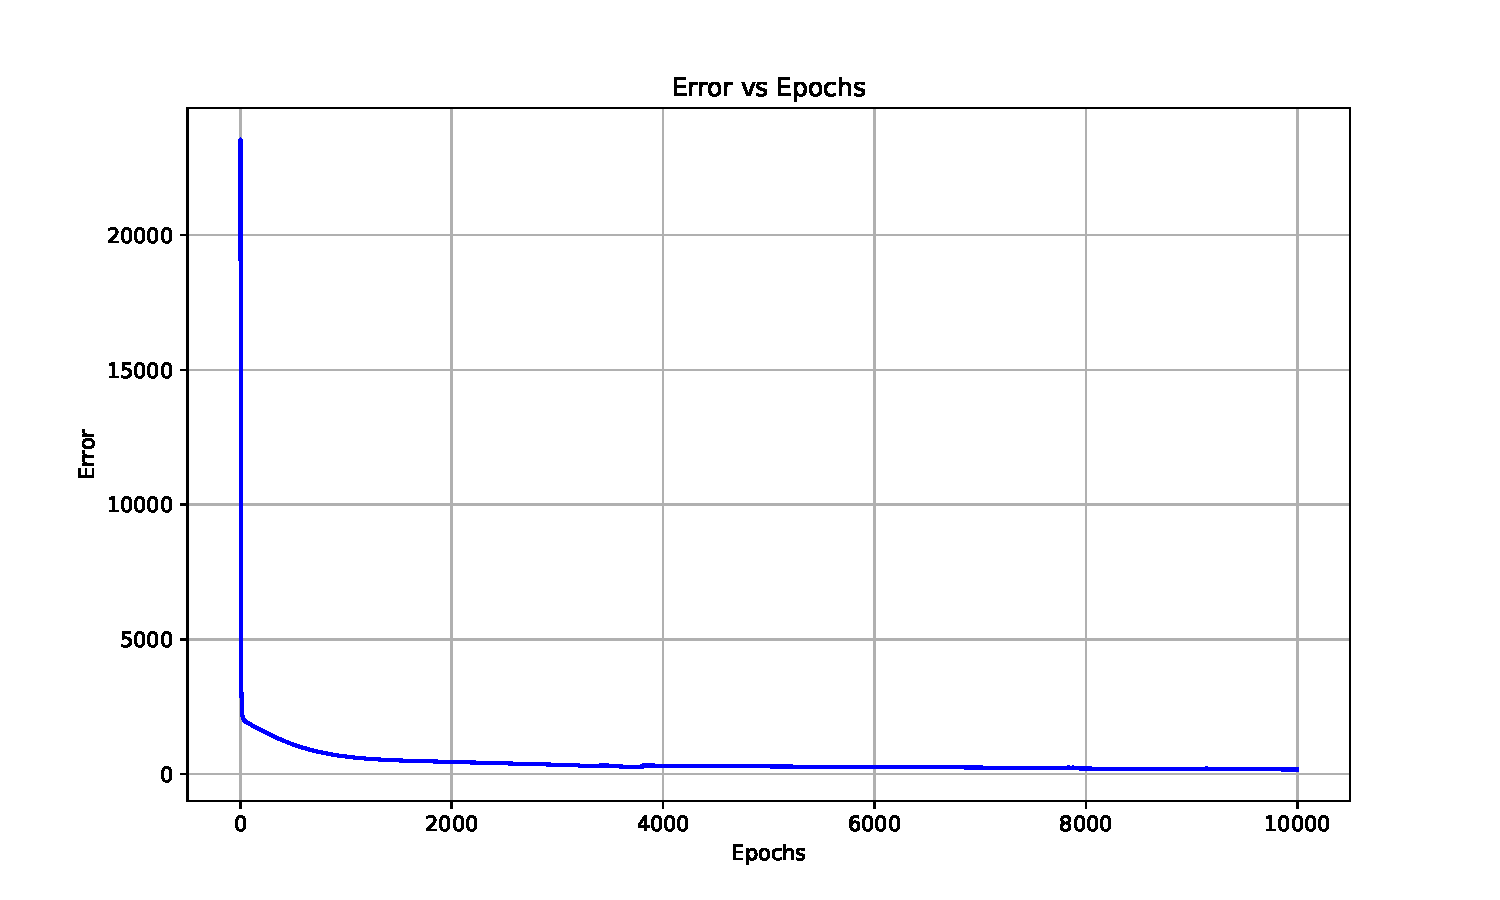
\includegraphics[width=0.8\textwidth, page=1]{pdfs/error_vs_epochs_0.1_10000_line_search.pdf}
    \caption{Error vs Epoch for Line Searching} 
    \label{fig:error_vs_epochsLS1}
\end{figure}

\begin{figure}[H]
    \centering
    \includegraphics[width=0.8\textwidth, page=2]{pdfs/error_vs_epochs_0.1_10000_line_search.pdf}
    \caption{Predicted vs Expected for Line Searching} 
    \label{fig:error_vs_epochsLS1}
\end{figure}

While the plots may be further away, the accuracy of the network is much higher, and the predictions at the first section of the year are much better.
This is a significant improvement and shows that the line search implementation is much more efficient.
However it is clear that their is an issue, as all the datapoints have been shifted upwards.
Once rectified, this will be the best implementation of the network.

\begin{figure}[H]
    \centering
    \includegraphics[width=0.8\textwidth, page=3]{pdfs/error_vs_epochs_0.1_10000_line_search.pdf}
    \caption{Skew for Line Searching} 
    \label{fig:error_vs_epochsLS1}
\end{figure}

After analysis, the model was overtraining as the batch size decreases.
By capping the batch size to 32, the model was able to learn more effectively and not overfit.
This is likely due to the line search being more effective with smaller batch sizes, and so the network was learning too much.

\begin{figure}[H]
    \centering
    \includegraphics[width=0.8\textwidth, page=2]{pdfs/error_vs_epochs_0.1_10000_linesearch3.pdf}
    \caption{Predicted vs Expected for Line Searching (2$^{nd}$ Implementation)} 
    \label{fig:error_vs_epochsLS1}
\end{figure}

\begin{figure}[H]
    \centering
    \includegraphics[width=0.8\textwidth, page=4]{pdfs/error_vs_epochs_0.1_10000_linesearch3.pdf}
    \caption{Correlation Plot for Line Searching (2$^{nd}$ Implementation)} 
    \label{fig:error_vs_epochsLS1}
\end{figure}

\chapter{Model training and testing}

Most model training and testing occured in the previous chapter, but we will now evaluate the best model and see how well it predicts the data.
\vspace{1em}
\newline
The best model was the line search model, with a batch size of 32.
This model was able to learn the most effectively and produce the best results in the quickest amount of time.
As all model simulations were done with the same random seed and with 10,000 epochs, the results may not be as good as they can be.
\vspace{1em}
\newline
We will take the model we chose and run it for 50,000 epochs and evaulate the error of the testing data to see how well the model predicts.

\begin{table}[H]
    \centering
    \begin{tabular}{|c|c|}
        \hline
        Time Taken (seconds) & Error (MSE)  \\
        \hline
        919 & 195 \\
        \hline
    \end{tabular}
    \caption{statistics for 50,000 epochs of Line Searching}
    \label{tab:dynamicMomentum}
\end{table}

When the model was trained for 50,000 epochs, the error was reduced to 195 on the evaluation data, which is a significant improvement.
It ended on an MSE of 141 on the training data, which is a significant improvement on previous models.
However, when run for 100,000 epochs, the model became overfit and the MSE increased to 1000 on the evaluation data.

\begin{figure}[H]
    \centering
    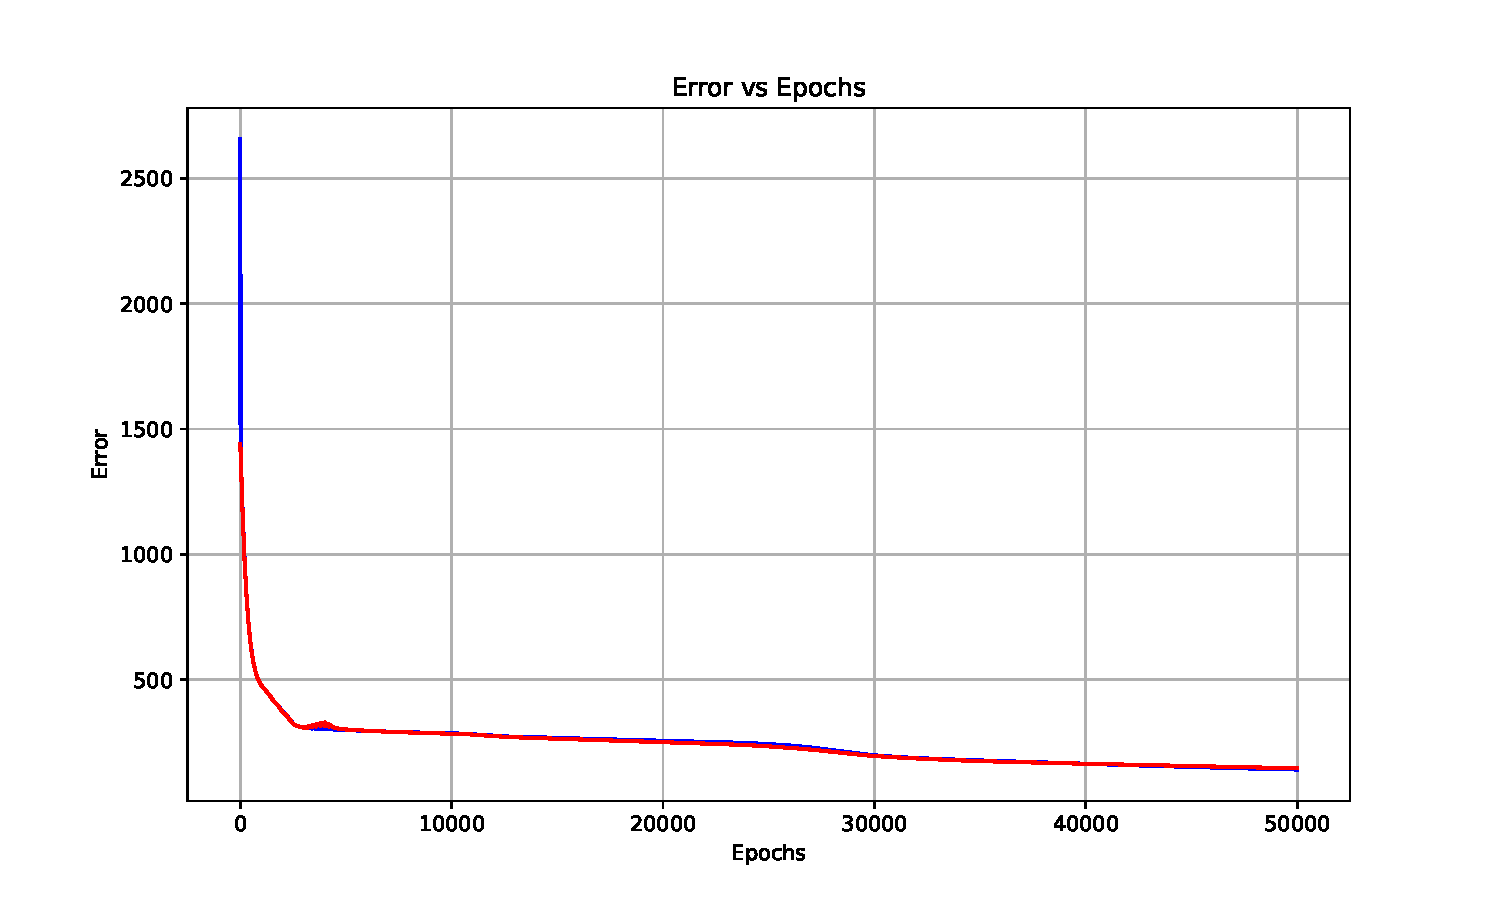
\includegraphics[width=0.8\textwidth, page=1]{pdfs/error_vs_epochs_0.1_50000_final.pdf}
    \caption{Error vs Epoch for Line Searching (50,000 epochs)} 
    \label{fig:error_vs_epochsLS1}
\end{figure}
The red line represents the error of the evaluation data, and the blue line represents the error of the training data.

\begin{figure}[H]
    \centering
    \includegraphics[width=0.8\textwidth, page=2]{pdfs/error_vs_epochs_0.1_50000_final.pdf}
    \caption{Predicted vs Expected for Line Searching (50,000 epochs)} 
    \label{fig:final_pred}
\end{figure}
The model matches very well to the expected output, and the correlation is very high for the steady data.
When the data becomes more sporadic, the model struggles with this

\begin{figure}[H]
    \centering
    \includegraphics[width=0.8\textwidth, page=6]{pdfs/error_vs_epochs_0.1_50000_final.pdf}
    \caption{Correlation Plot for Line Searching (50,000 epochs)} 
    \label{fig:final_corr}
\end{figure}


\chapter{Evaluation}

\section{Model Evaluation}
The provided model was able to predict the error with a mean squared error of 195, and a time of 919 seconds
The development of the model was costly, and the time taken to train the model was significant.

\begin{figure}[H]
    \centering
    \includegraphics[width=0.8\textwidth, page=4]{pdfs/error_vs_epochs_0.1_50000_final.pdf}
    \caption{Predicted vs Expected for Line Searching (50,000 epochs)} 
    \label{fig:final_pred}
\end{figure}
The predicted evaluation data is shown in red, and the expected evaluation data is shown in blue.
It is obvious that the model is not able to predict the sporadic data as well as the steady data, however the model is acceptable.
The MSE of 195 gives an average difference of 14, which clearly takes more affect at the sporadic data.

\section{Model Comparison}
We can compare the model with a basic linear regression algorithm to see how well the model performs.
This will allow us to see how well the model performs compared to a simple model.

\begin{table}[H]
    \centering
    \begin{tabular}{|c|c|}
        \hline
        Time Taken (seconds) & Error (MSE)  \\
        \hline
        0.17 & 119 \\
        \hline
    \end{tabular}
    \caption{statistics for Linear Regression}
    \label{tab:linregres}

\end{table}

The linear regression model beats the neural network model in both metrics.
This is likely because there is a largely linear relationship between the inputs and output, and so a linear regression model is the best model for this data.
All 7 inputs are highly correlated and it intuitively follows that they have a high linear correlation.

\begin{figure}[H]
    \centering
    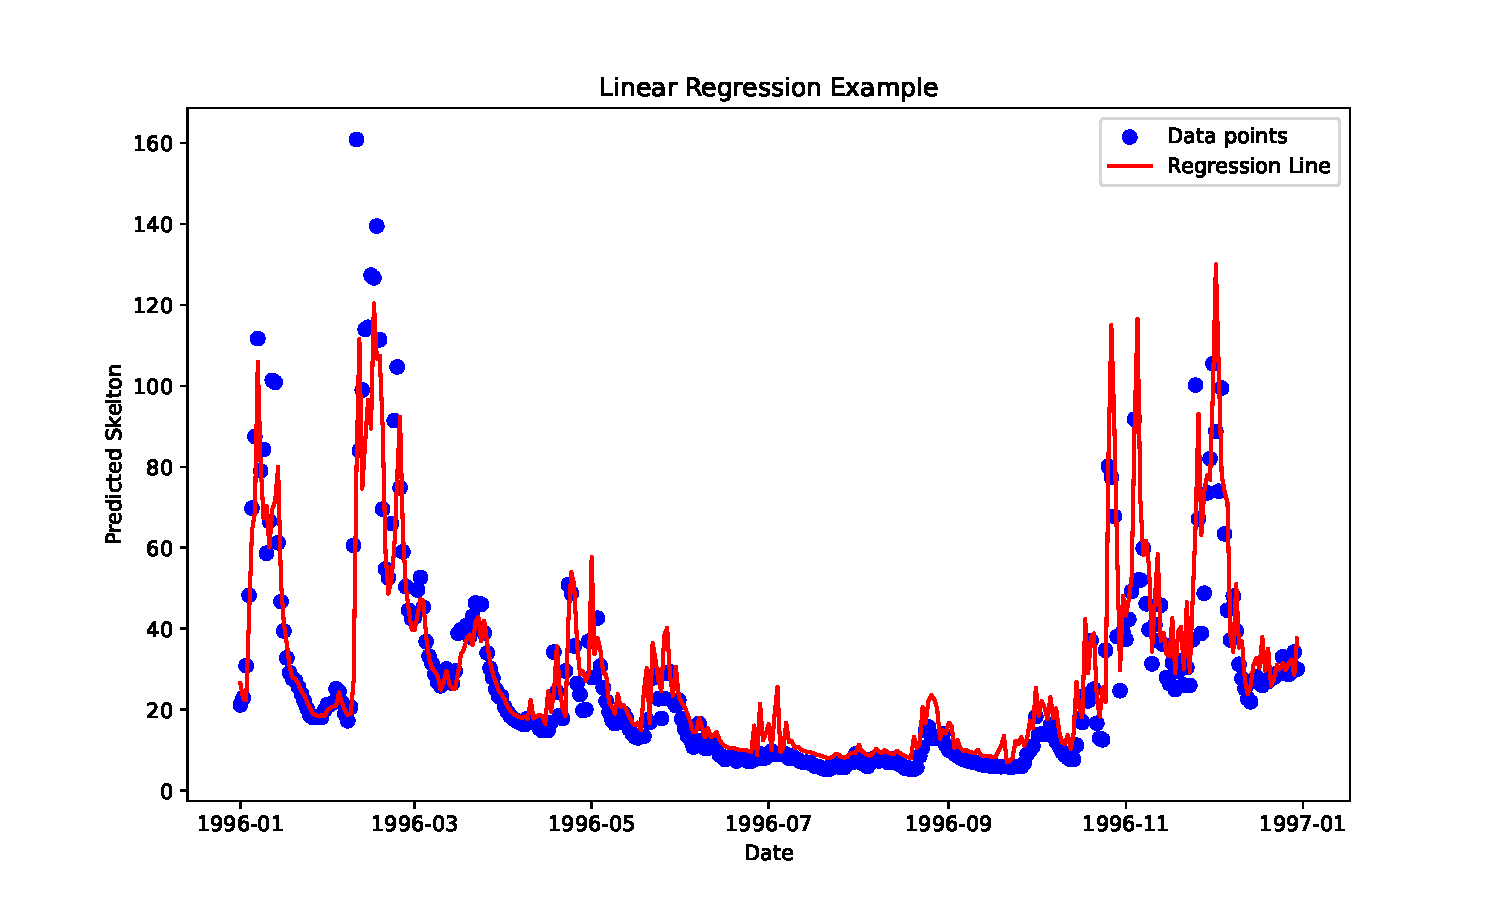
\includegraphics[width=0.8\textwidth, page=1]{pdfs/lin_regression.pdf}
    \caption{Expected vs Predicted for Linear Regression} 
    \label{fig:error_vs_epochsLS1}
\end{figure}

The linear regression model is able to predict the data very well, with a MSE of 119.
This means that the average difference is 11 between the expected and predicted data.
This is a significant improvement on the neural network model, but mainly interms of time and effort.
\vspace{1em}
\newline
A differnce of 11 and 14 is not a significant difference, but the time taken to train the model is.

\section{Conclusions}
The neural network model is able to predict the data well. It used 50\% of the data and trained for 50,000 epochs.
With the chosen model this was a 195 MSE on the final evaluation data. 
I would conclude that this neural network is an effective way of predicting the data, but it is not the best way.
\vspace{1em}
\newline
The linear regression model is able to predict the data better, with a 119 MSE on the final evaluation data.
The linear regression model takes only 0.17 seconds to train, which is significantly faster than the neural network model, around 6000 times faster.
While the training time is faster, so is the amount of time spent developing the model.
\vspace{1em}
\newline
In conclusion, the Linear Regression model is the best model for this data, as it is able to predict the data better and faster than the neural network model.

\section{Potential Improvements}
If I was to improve my network, I would try to work with different structures and optimise there.
I only used 1 Cost funciton and 1 Activation function, and so I could try different ones to see if they are more effective.
I could also try to vary the node structure and see if that is more effective with more layers or nodes.
I could also try to implement a seperate gradient calculation, such as conjufate gradient searching.
\vspace{1em}
\newline
Overall I am please with my results and for this purpose, The model is effective and efficient.

\section{Extra Plots}
\begin{figure}[H]
    \centering
    \includegraphics[width=0.8\textwidth, page=5]{pdfs/error_vs_epochs_0.1_50000_final.pdf}
    \caption{Predicted vs Expected for Line Searching  (50,000 epochs)} 
    \label{fig:final_pred}
\end{figure}
Predicted vs Expected for the whole given dataset.

\begin{figure}[H]
    \centering
    \includegraphics[width=0.8\textwidth, page=8]{pdfs/error_vs_epochs_0.1_50000_final.pdf}
    \caption{Correlation for Line Searching  (50,000 epochs)} 
    \label{fig:final_pred}
\end{figure}
Correlation between predicted and expected data for the whole given dataset.

\end{document}
 

